\section{Background studies with minimum bias Monte Carlo}

In order to better understand the combinatoric background, minimum bias Monte Carlo files\footnote{The files can be found in the LHCb bookkeeping under the references \texttt{/MC/2012/30000000/Beam4000GeV-2012-MagUp-Nu2.5-Pythia8/Sim08a/Digi13/Trig0x409f0045/\\Reco14a/Stripping20NoPrescalingFlagged/ALLSTREAMS.DST},\\\texttt{/MC/2012/30000000/Beam4000GeV-2012-MagDown-Nu2.5-Pythia8/Sim08a/Digi13/Trig0x409f0045/\\Reco14a/Stripping20NoPrescalingFlagged/ALLSTREAMS.DST},\\\texttt{/MC/2012/30000000/Beam4000GeV-2012-MagUp-Nu2.5-Pythia8/Sim08c/Digi13/Trig0x409f0045/\\Reco14a/Stripping20NoPrescalingFlagged/ALLSTREAMS.DST}, and \\\texttt{/MC/2012/30000000/Beam4000GeV-2012-MagDown-Nu2.5-Pythia8/Sim08c/Digi13/Trig0x409f0045/\\Reco14a/Stripping20NoPrescalingFlagged/ALLSTREAMS.DST}.} have been processes with the same selections as described in section \ref{SEC:Efficiencies}.  From the 42 million input events, those that remain after the selection have the following background categories:
\begin{center}
\begin{tabular}{c|c|c}
Background category & Prompt $\phi$ & $D_s \rightarrow \phi \pi$ \\ 
\hline 
light flavour & 17(17) & 0 \\ 
$b\overline{b}$ & 1(1) & 0 \\ 
different PV & 3(2) & 0 \\ 
physical bkg, partl. reconstructed & 1(1) & 1(1) \\ 
ghosts & 0 & 1(0) \\ 
\hline 
total & 21(20) & 2(1) \\  
\end{tabular} 
\captionof{table}{Background categories of the minimum bias Monte Carlo events remaining after the selection. The number in brackets is the number of background events with true $K_S$.}
\end{center}

It can be concluded that 80\% of the background after the prompt $\phi$ selection is prompt $K_S$ originating from the primary vertex. For the $D_s^\pm \rightarrow \phi\pi^\pm$ selection, the number of events in the Monte Carlo sample is too low to gain more information about the background types.

\section{Time resolution}
Since CPT violation would be visible as an excess of $\phi \rightarrow K^0 \overline{K}^0 \rightarrow \pi^+ \pi^- \pi^+ \pi^-$ for small $\Delta t$, knowledge about the time resolution of the detector for this system is important.
Two differenent methods have been considered for the reconstruction of the decay times. 
The first uses the DaVinci class TupleToolPropertime %\footnote{\url{http://lhcb-release-area.web.cern.ch/LHCb-release-area/DOC/rec/releases/v14r2/doxygen/d3/df5/class_tuple_tool_propertime.html}} 
to determine the decay times from the reconstructed particles. The standard reconstruction follows a bottom-up approach, starting with parameters of the reconstructed final state particles and then working its way up by determining the parameters of each mother particle via a fit to those parameters of its daughter particles \cite{2005NIMPA.552..566H}.
The second method uses the DecayTreeFitter %\footnote{\url{https://lhcb-release-area.web.cern.ch/LHCb-release-area/DOC/hlt/latest_doxygen/df/d04/namespace_decay_tree_fitter.html}}.
which performs a simultaneous fit of all vertices \cite{2005NIMPA.552..566H}. For this study, in this fit, the kaon mass was constrained to the nominal $K_S$ mass.


To determine the resolution, the reconstructed decay times $t(\text{reconstructed})$ were compared with the true decay times $t(\text{true})$ for the $D_S^\pm \rightarrow \phi \pi^\pm$ and the prompt $\phi$ Monte Carlo, the different figures being presented next to each other in the following.


\subsection{Using the DecayTreeFitter}
The DecayTreeFitter does not allow for negative decay times. Therefore 
\begin{equation}
t(\text{reconstructed})-t(\text{true})\geq - t(\text{true}),
\end{equation}
which leads to a sharp edge for negative residuals as illustrated for LL kaons in figure \ref{FIG:LL-DTF}. 

The resolution was estimated by fitting the residual for those cases where $t(\text{reconstructed})-t(\text{true}) \geq 0$ to a Breit Wigner distribution
\begin{equation}
N(\delta t) = \frac{a}{(\delta t- \mu)^2 - \Gamma^2/4}, \qquad \delta t = t(\text{reconstructed})-t(\text{true}) \label{EQ:BWt}
\end{equation}
as shown in figure \ref{FIG:timeres-LL-DTF}. For this specific fit, the centre was fixed to $\mu =0$.

\begin{center}
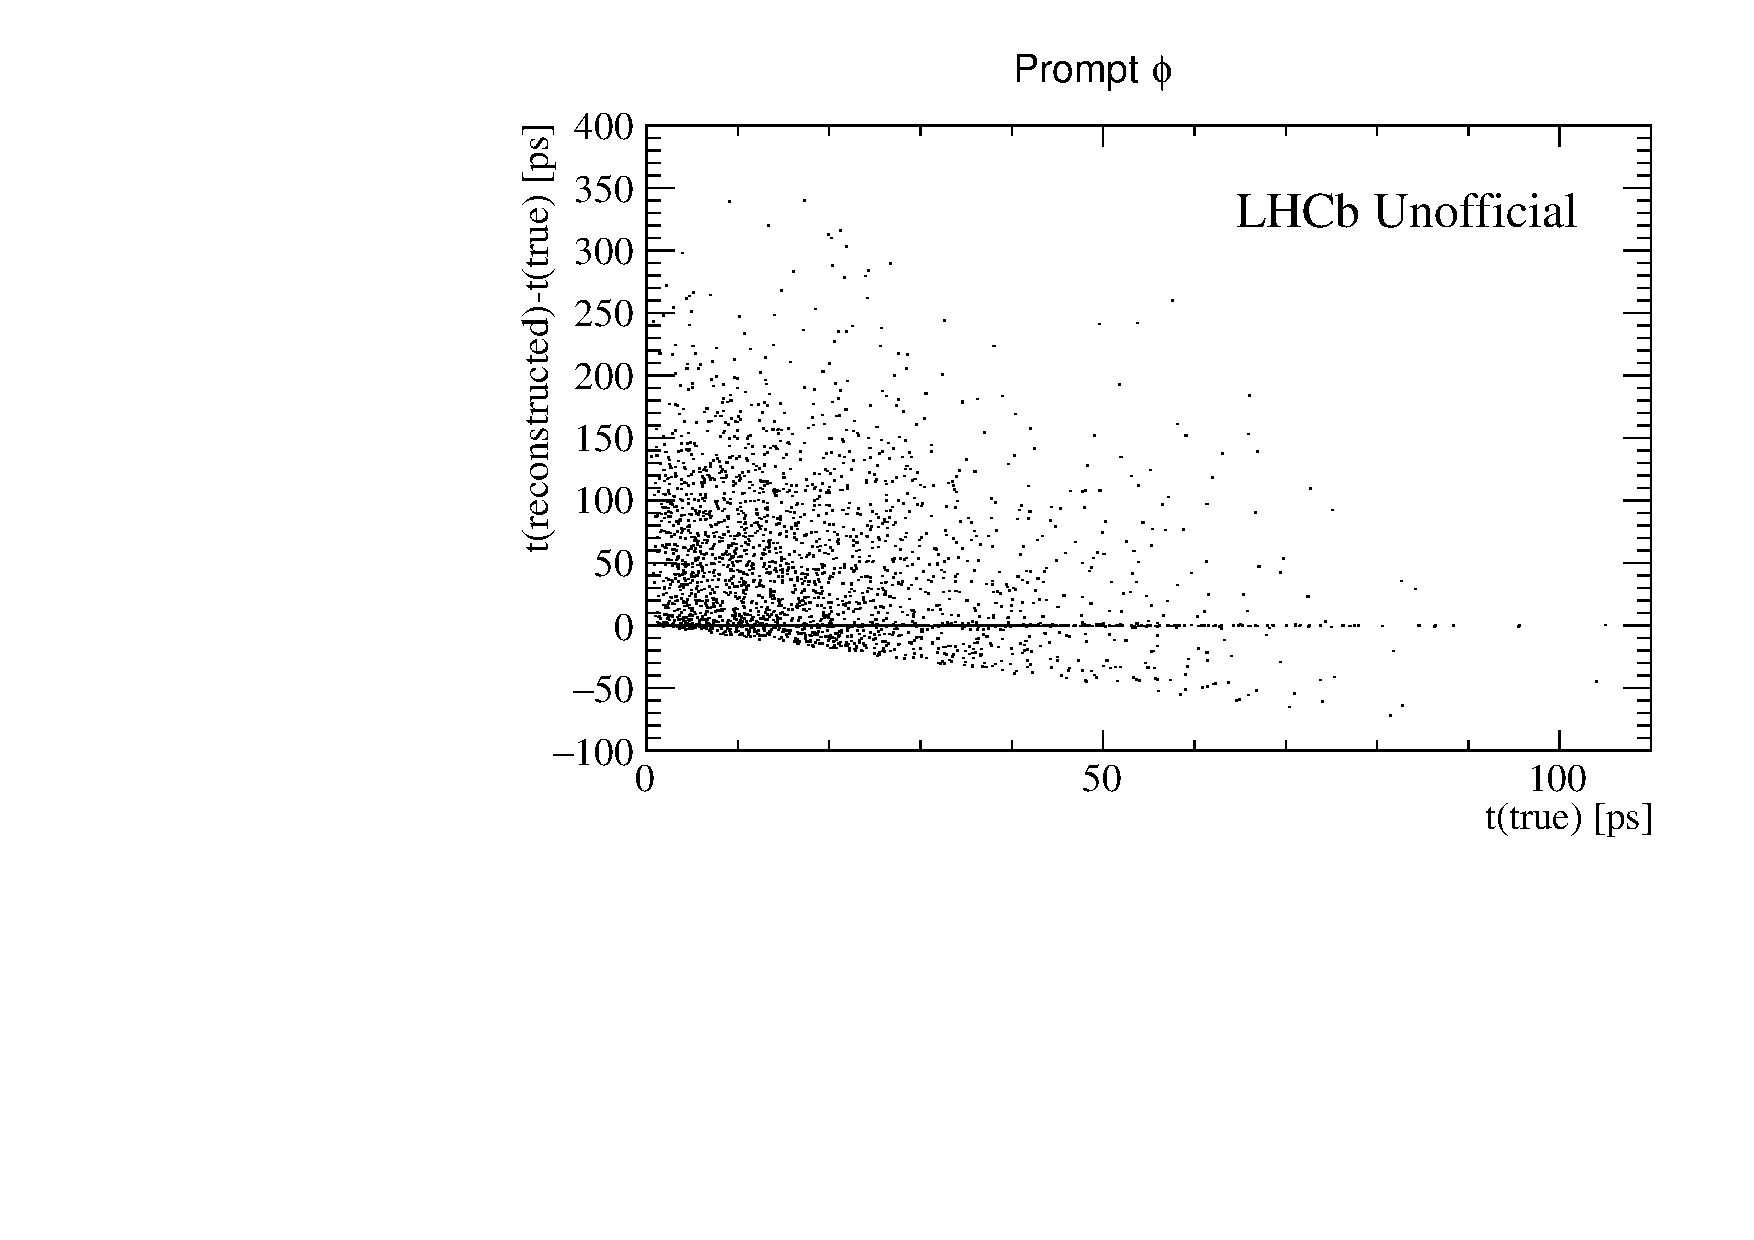
\includegraphics[width=.49\textwidth]{figs/time_res_incl/LL-DTF.pdf}
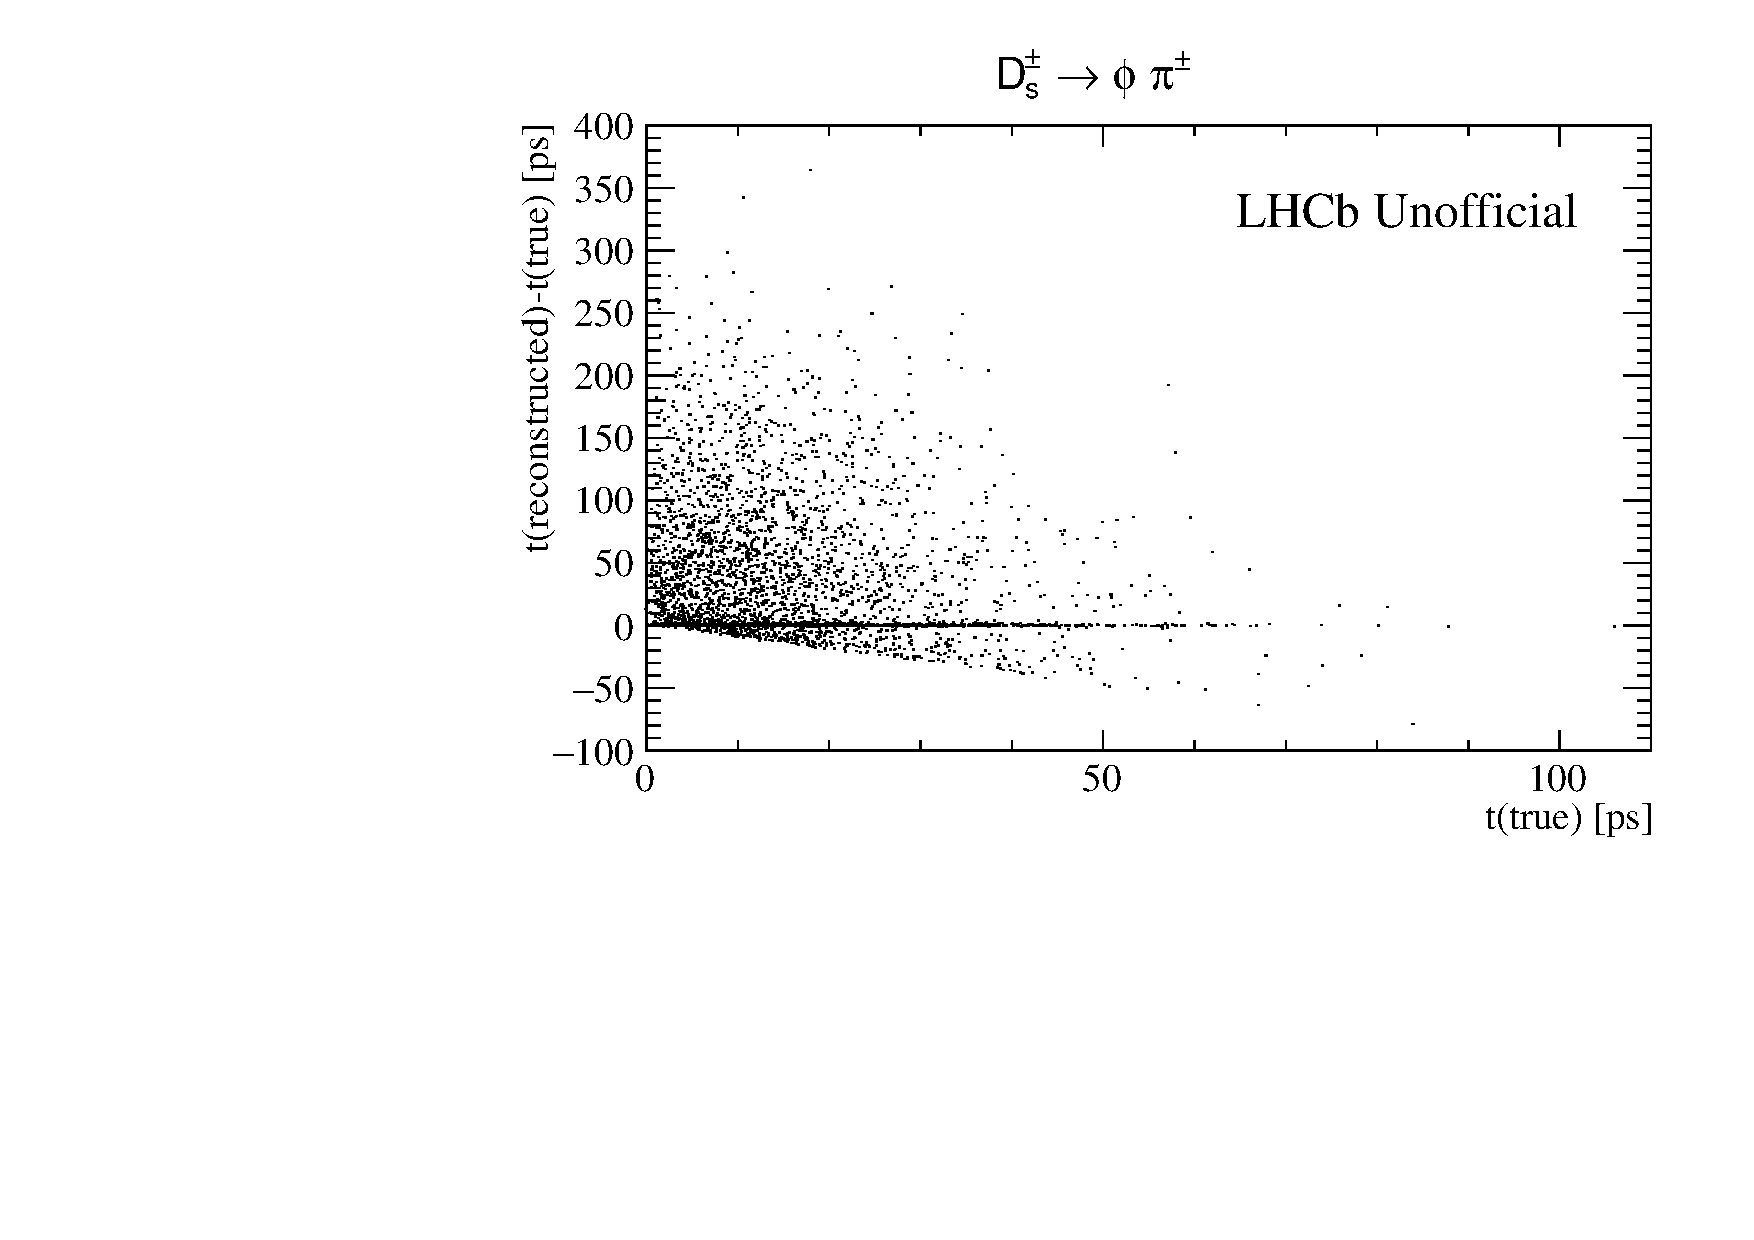
\includegraphics[width=.49\textwidth]{figs/time_res_Ds/LL-DTF.pdf}
\captionof{figure}{Residual of $t$ for LL kaons reconstructed via DecayTreeFitter plotted against the true value of $t$. }\label{FIG:LL-DTF}


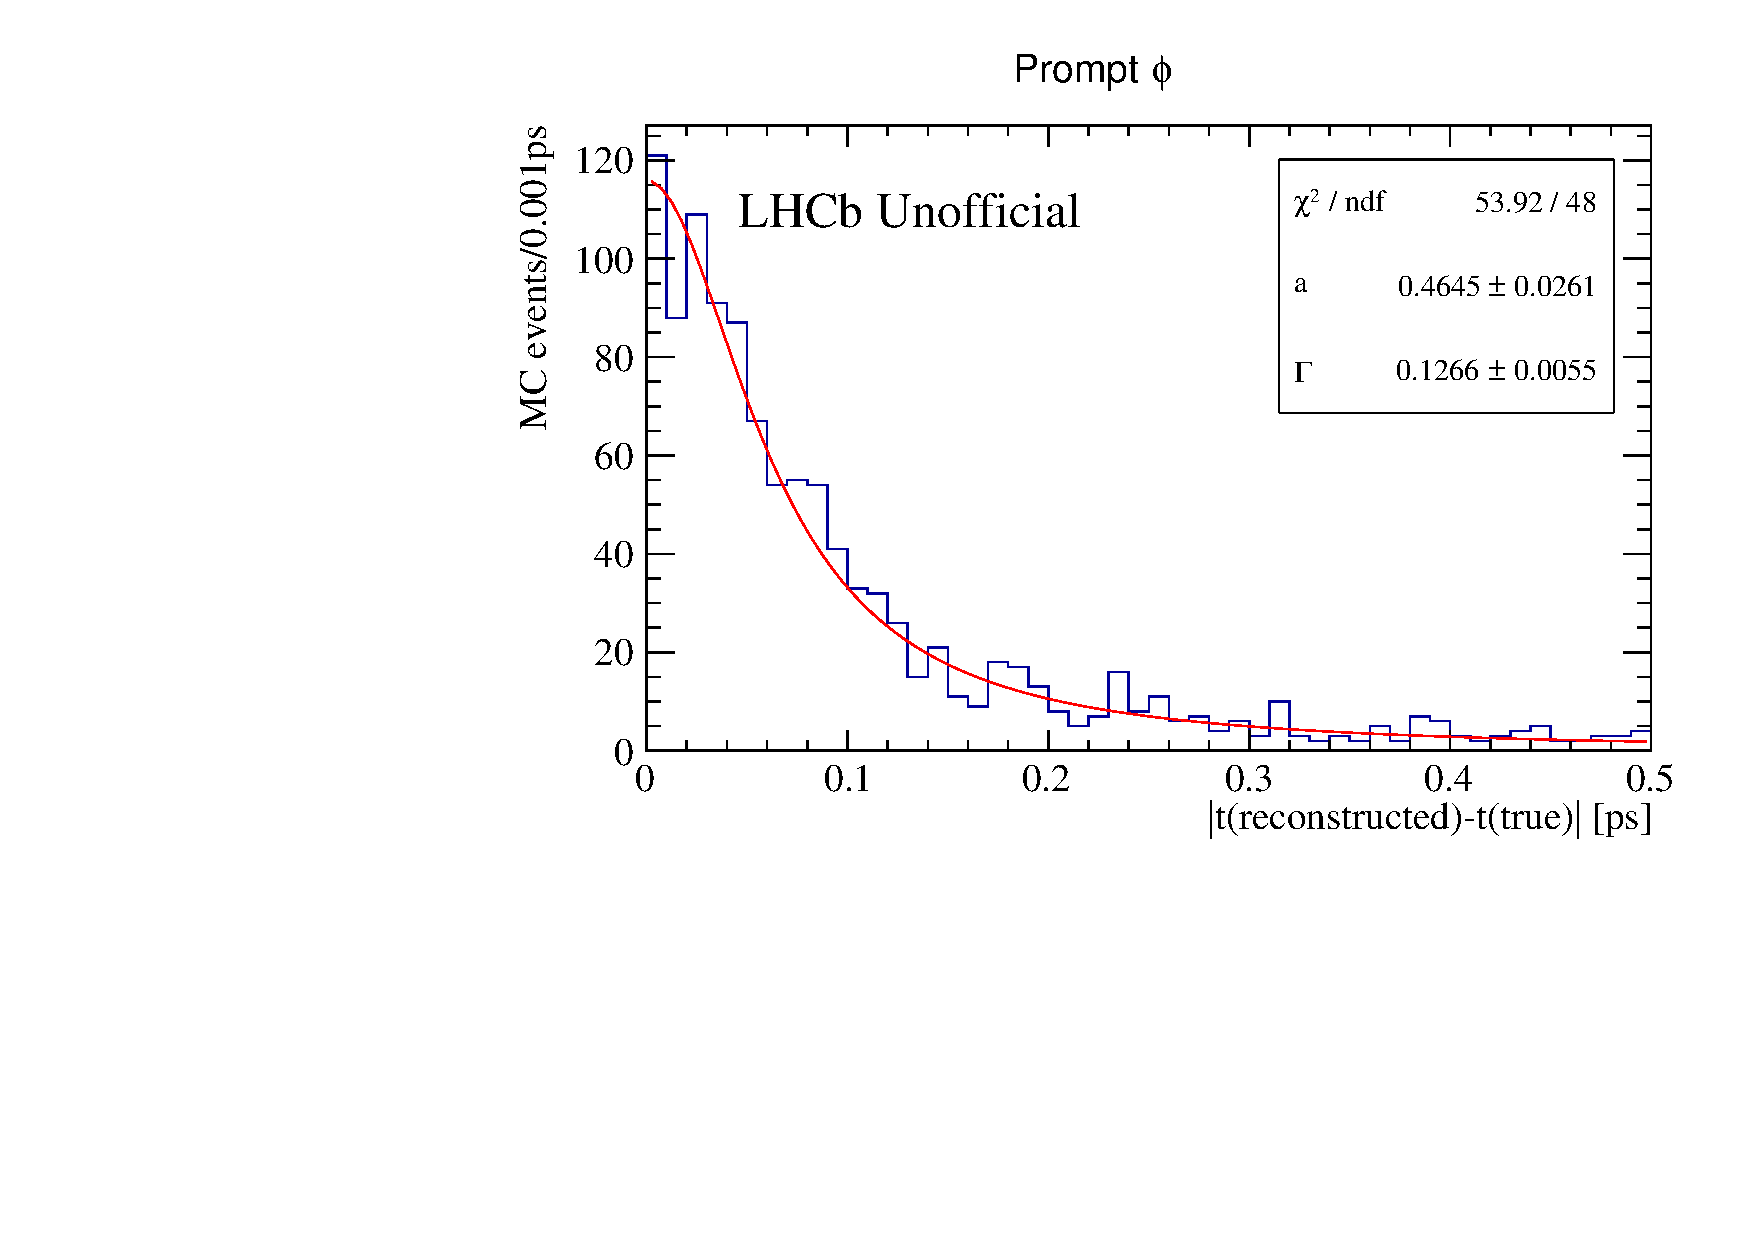
\includegraphics[width=.49\textwidth]{figs/time_res_incl/timeResolution-LL-DTF.pdf}
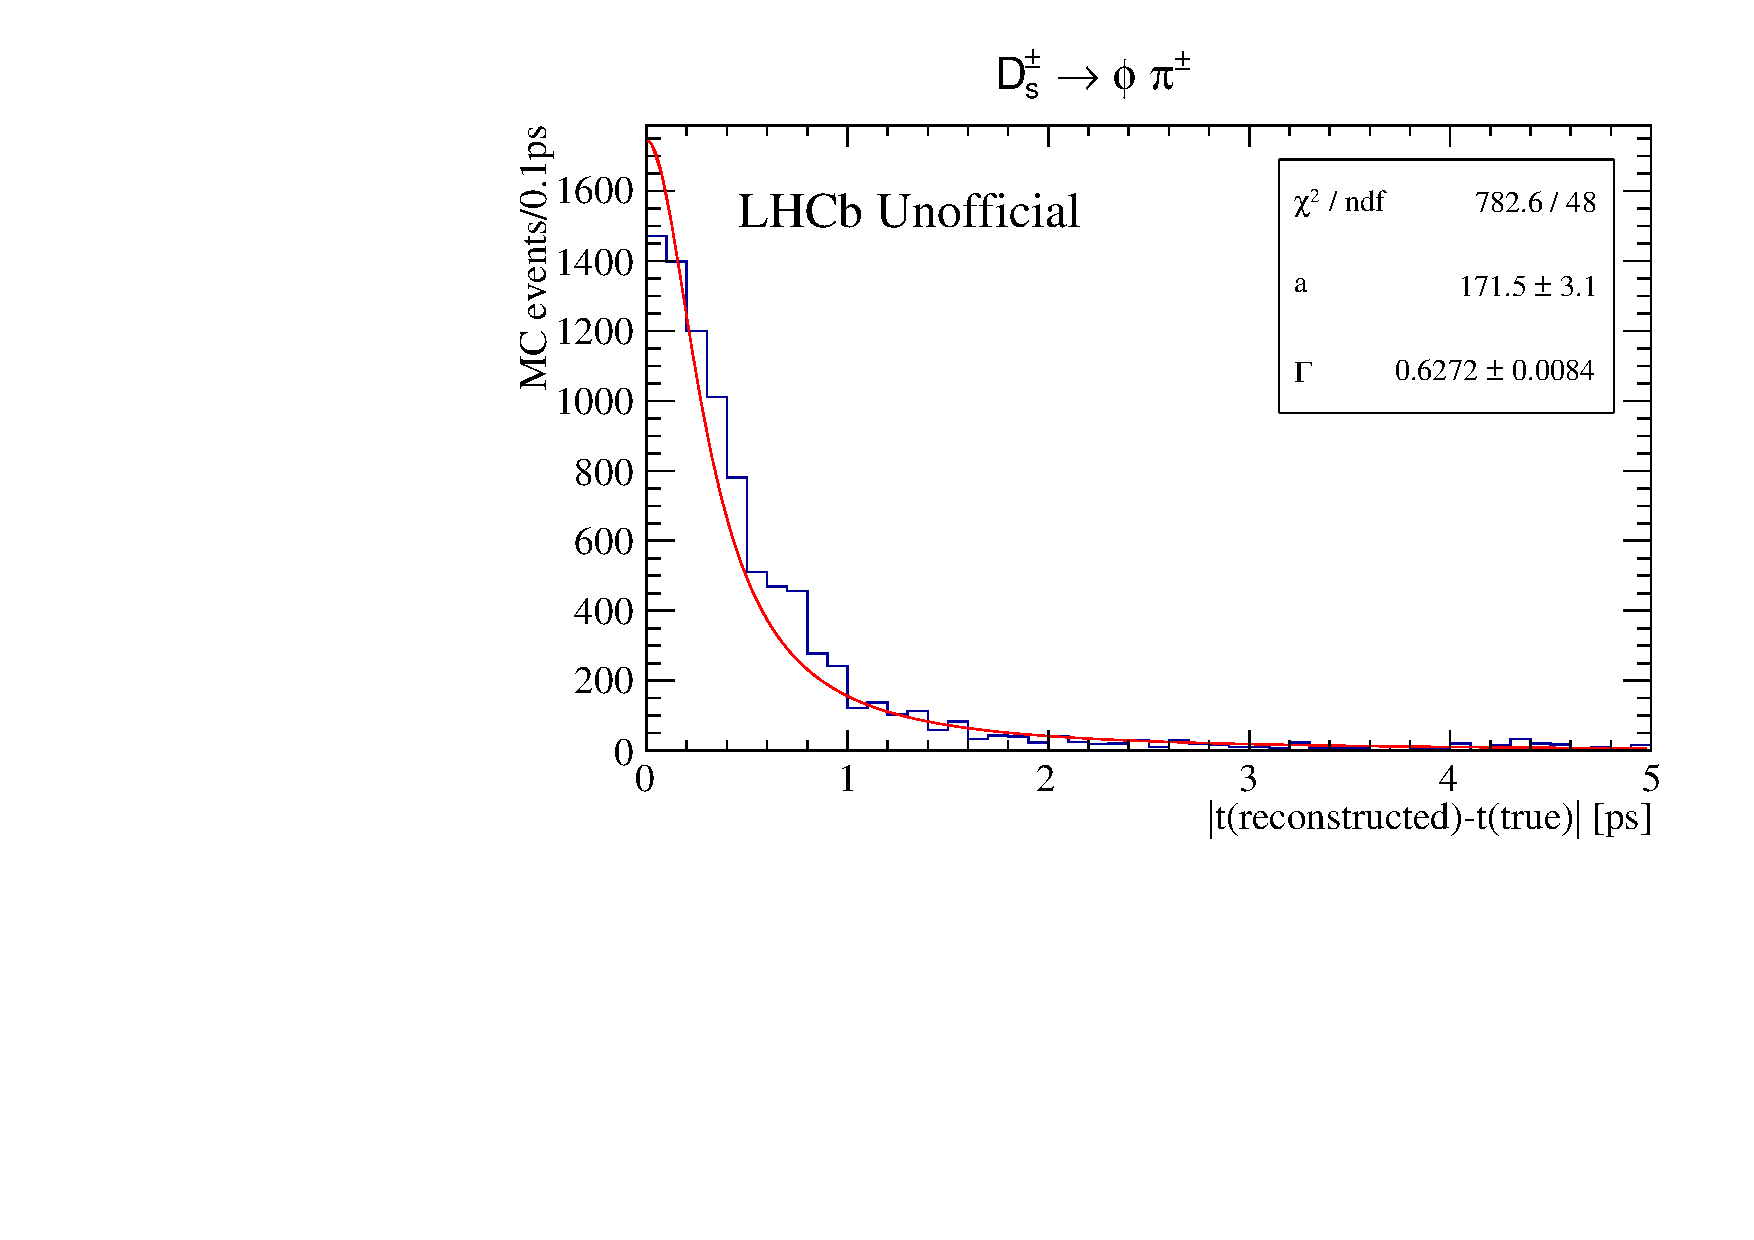
\includegraphics[width=.49\textwidth]{figs/time_res_Ds/timeResolution-LL-DTF.pdf}
\captionof{figure}{Resolution of LL kaon decay times $t$ reconstructed via the DecayTreeFitter. }\label{FIG:timeres-LL-DTF}


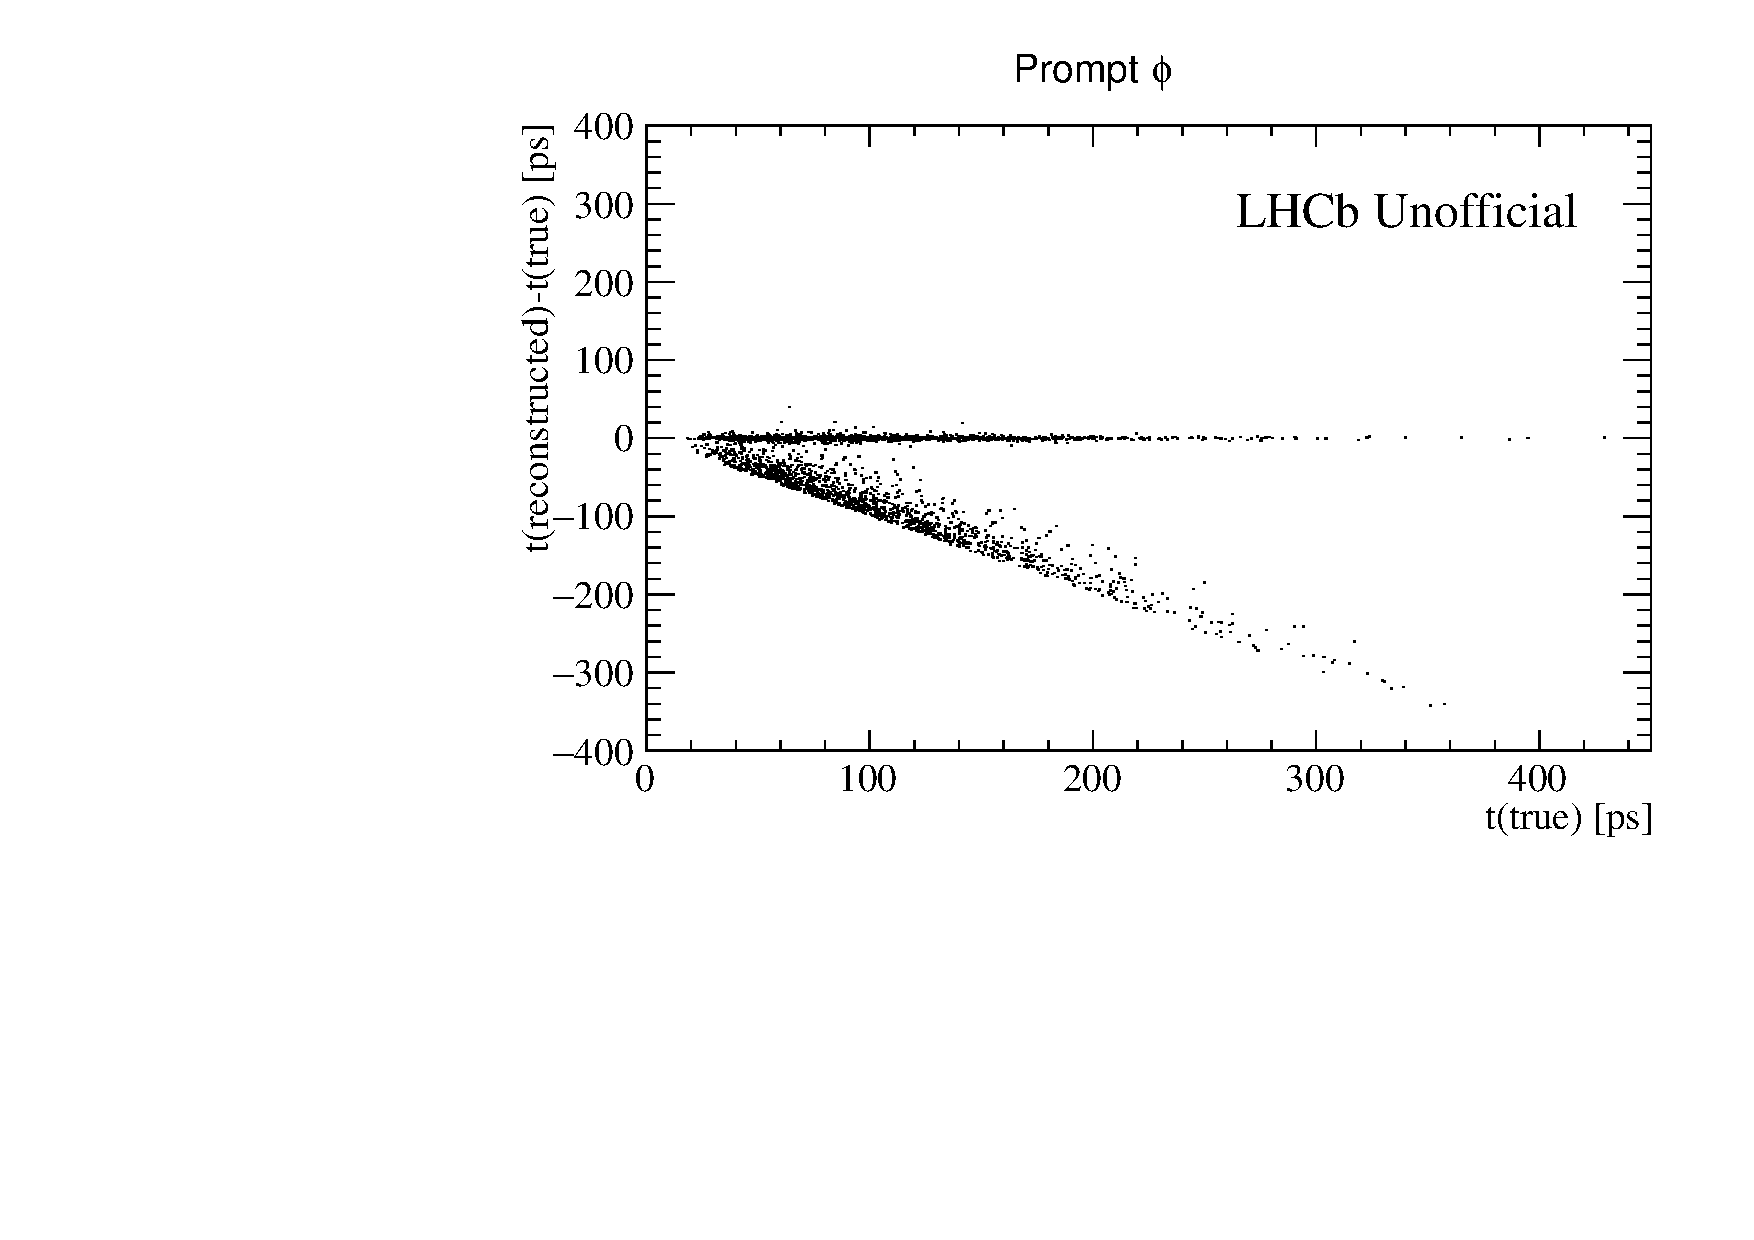
\includegraphics[width=.49\textwidth]{figs/time_res_incl/DD-DTF.pdf}
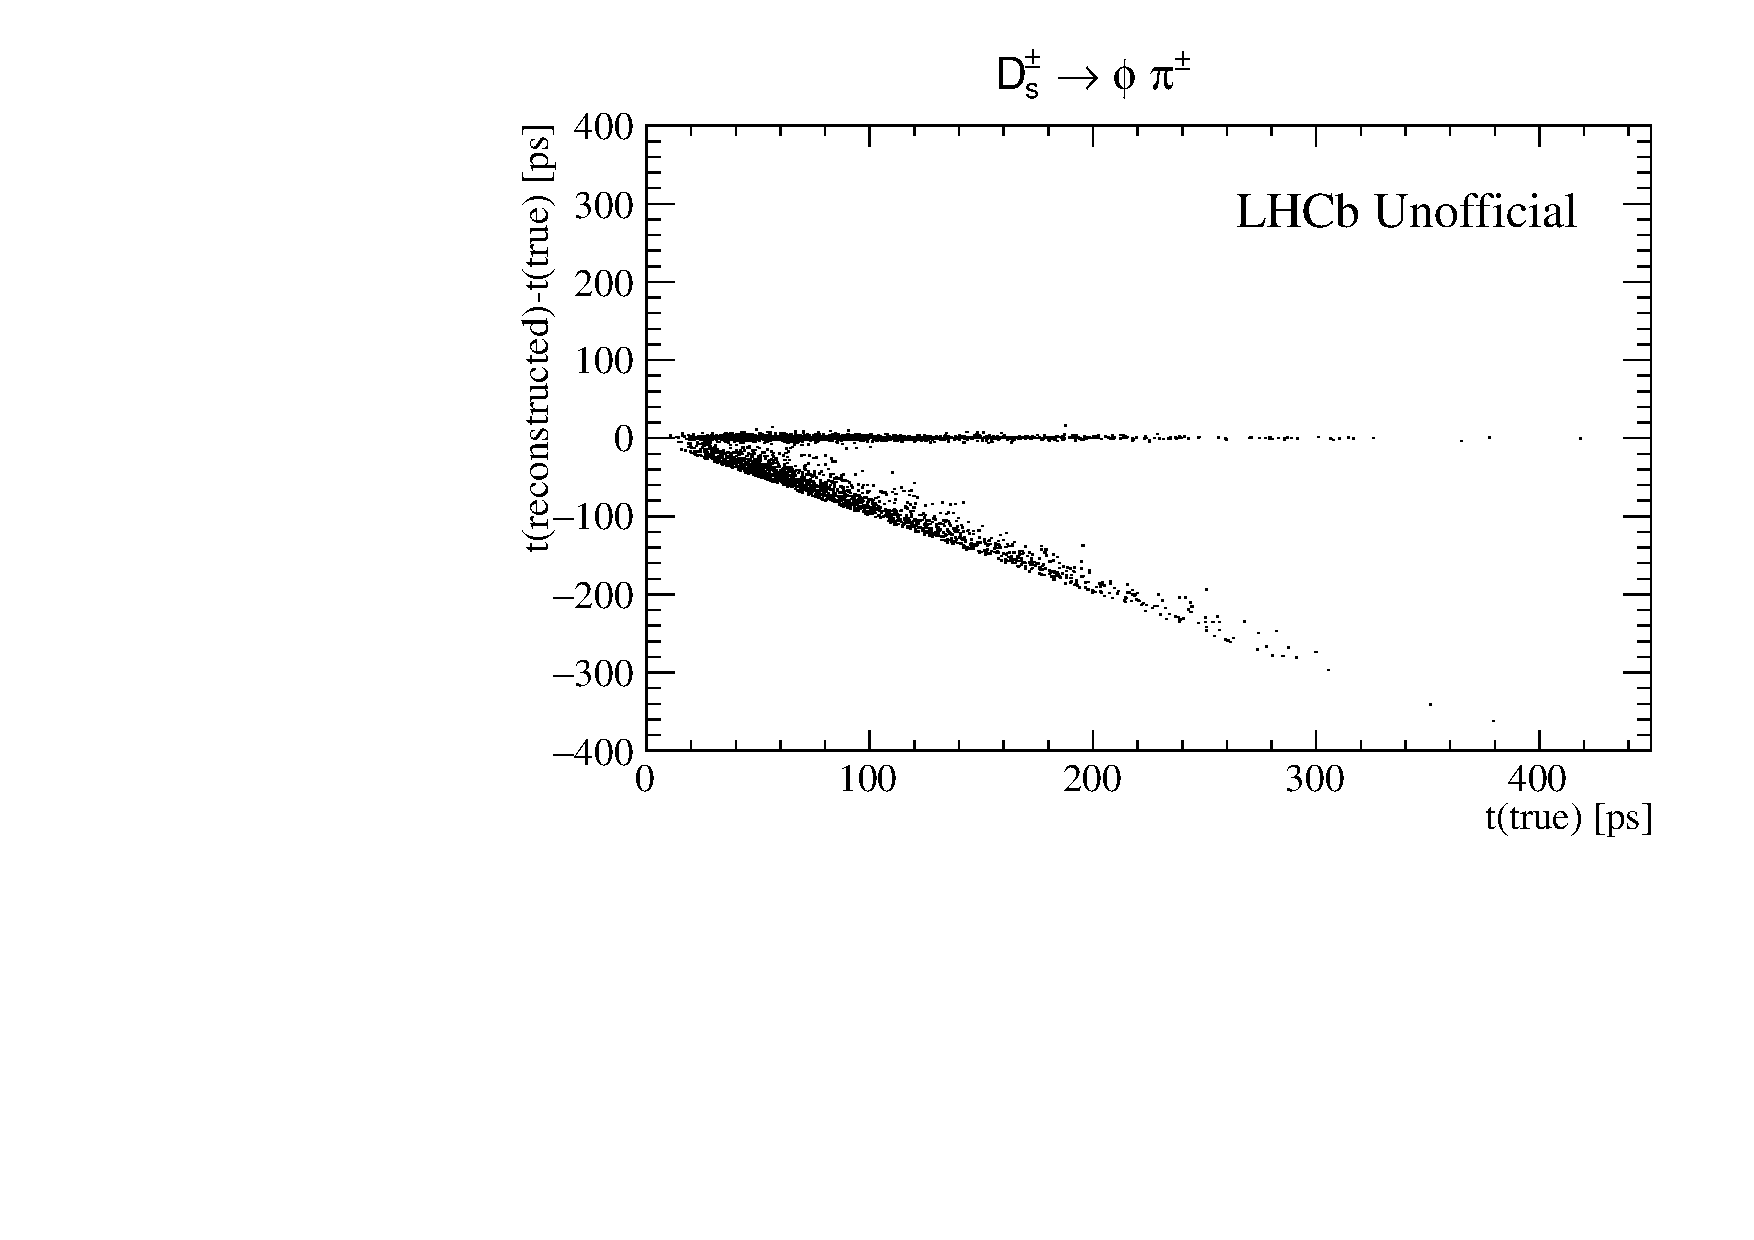
\includegraphics[width=.49\textwidth]{figs/time_res_Ds/DD-DTF.pdf}
\captionof{figure}{Residual of $t$ for DD kaons reconstructed via DecayTreeFitter plotted against the true value of $t$. }\label{FIG:DD-DTF}

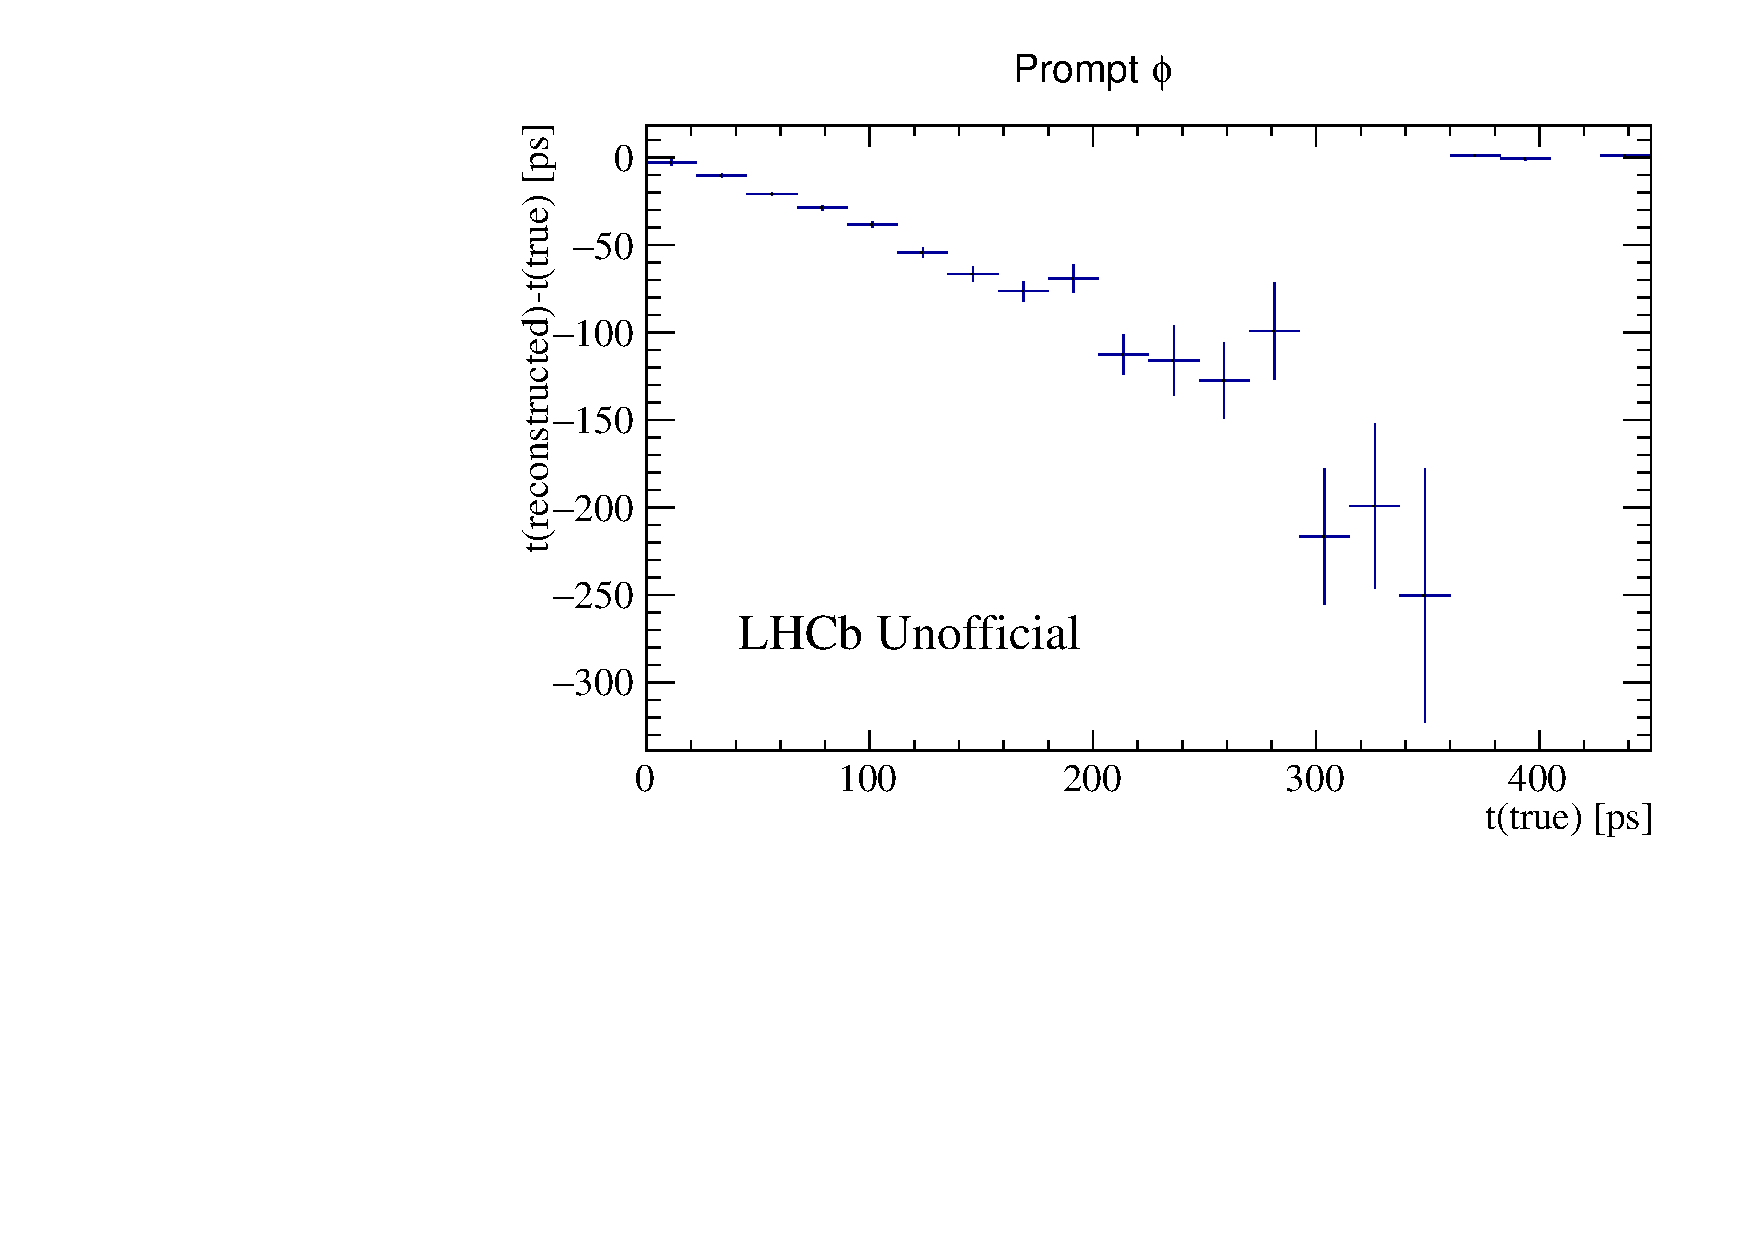
\includegraphics[width=.49\textwidth]{figs/time_res_incl/DD-DTF-prof.pdf}
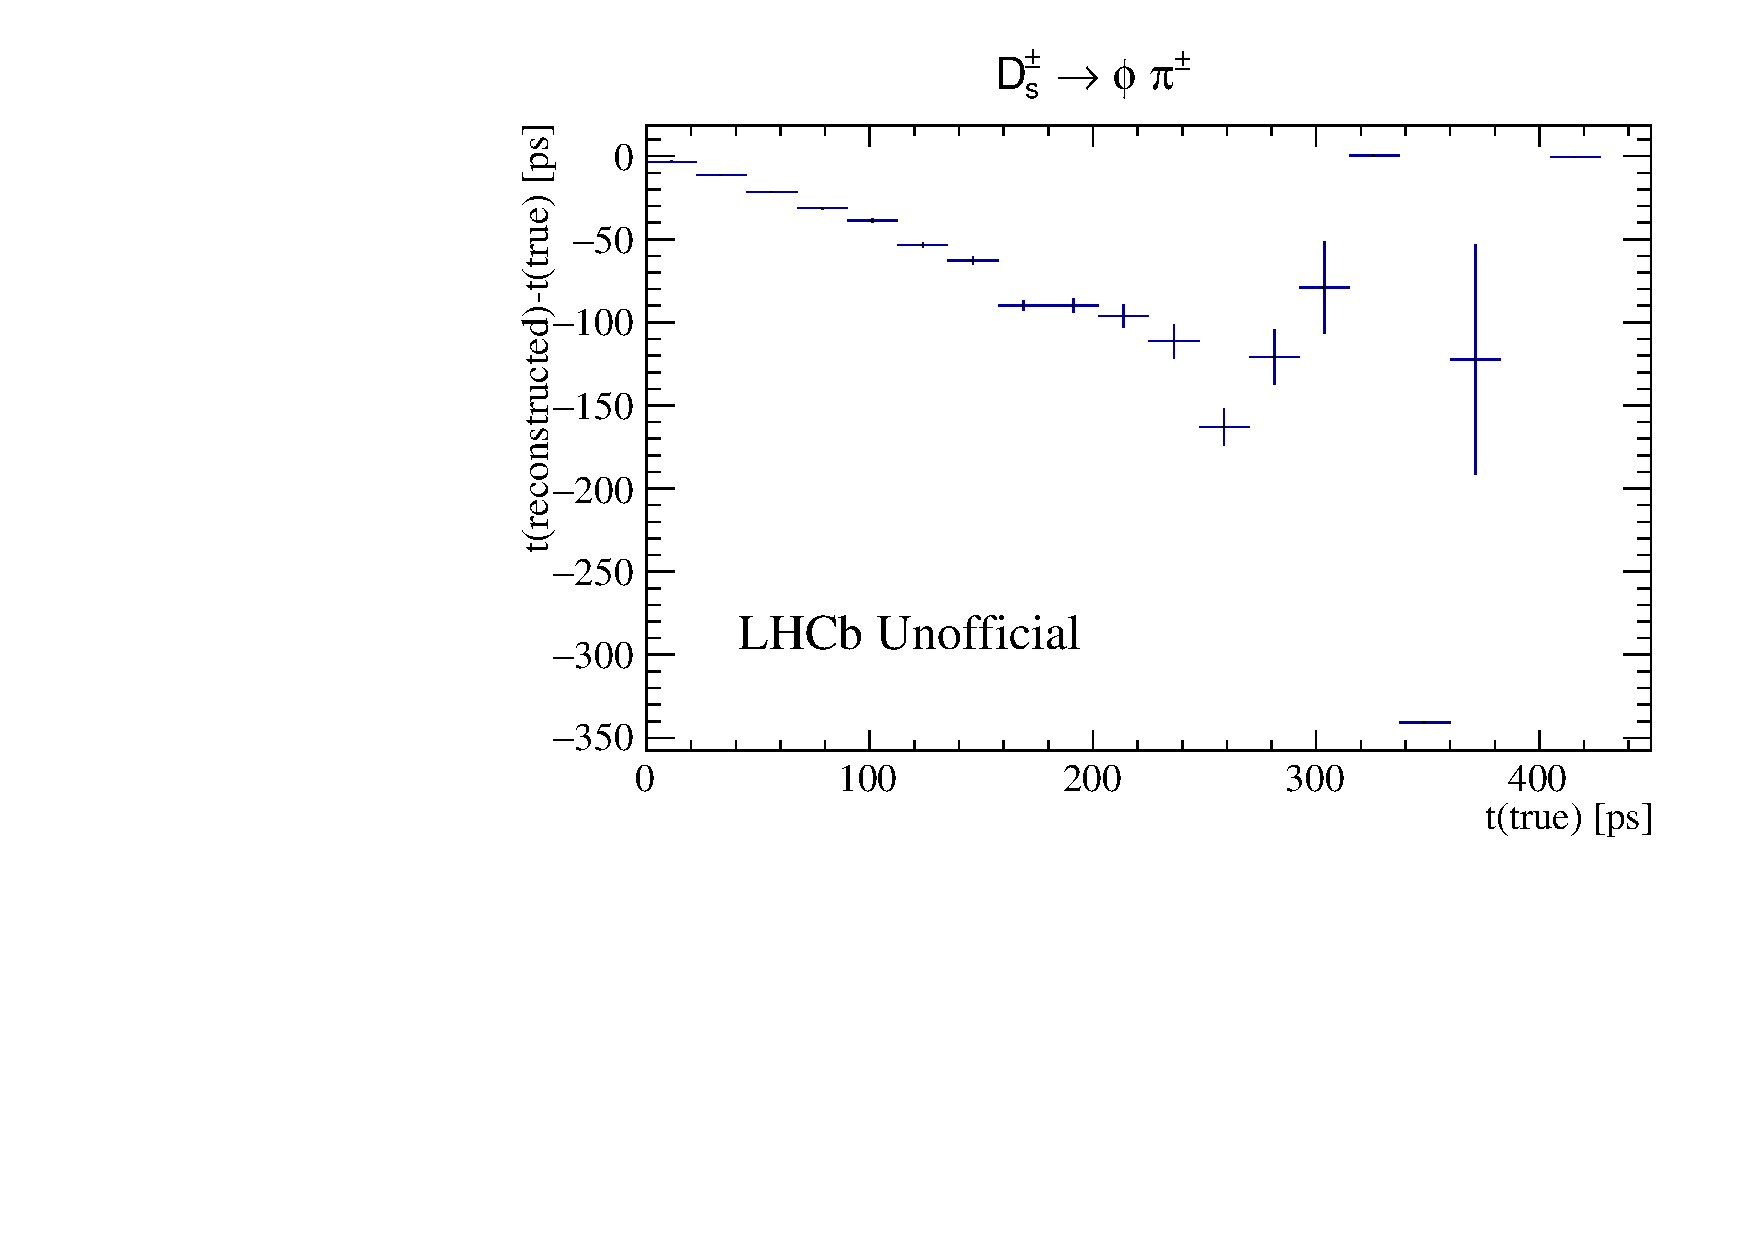
\includegraphics[width=.49\textwidth]{figs/time_res_Ds/DD-DTF-prof.pdf}
\captionof{figure}{Average residual of $t$ for DD kaons reconstructed via DecayTreeFitter plotted against the true value of $t$. }\label{FIG:DD-DTF-prof}
\end{center}


For DD kaons, sensitivity on the decay times is not given because the DecayTreeFitter sometimes reconstructs the decay times of the kaons as close to zero, maybe due to a lack of information available, which can be seen in figure \ref{FIG:DD-DTF}. This results in an underestimation of the decay times as shown in figure \ref{FIG:DD-DTF-prof}.
Therefore it is not advised to use the DecayTreeFitter in the context of decay time reconstruction with downstream tracks.

Since for probing the CPT invariance of the system, the observable $\Delta t = |t_1 - t_2|$ is used, its resolution for LL kaons has been studied as well, as it is displayed in figure \ref{FIG:timres-LL-DTF-prof}. To do this, the residual $\delta(\Delta t)$ has been fitted to the Breit Wigner distribution 
\begin{equation}
N(\delta(\Delta t)) = \frac{a}{(\delta(\Delta t)- \mu)^2 - \Gamma^2/4}. \label{EQ:BWdeltat}
\end{equation}
All resolution widths for LL kaons are given in table \ref{TAB:DTF}.
\begin{center}
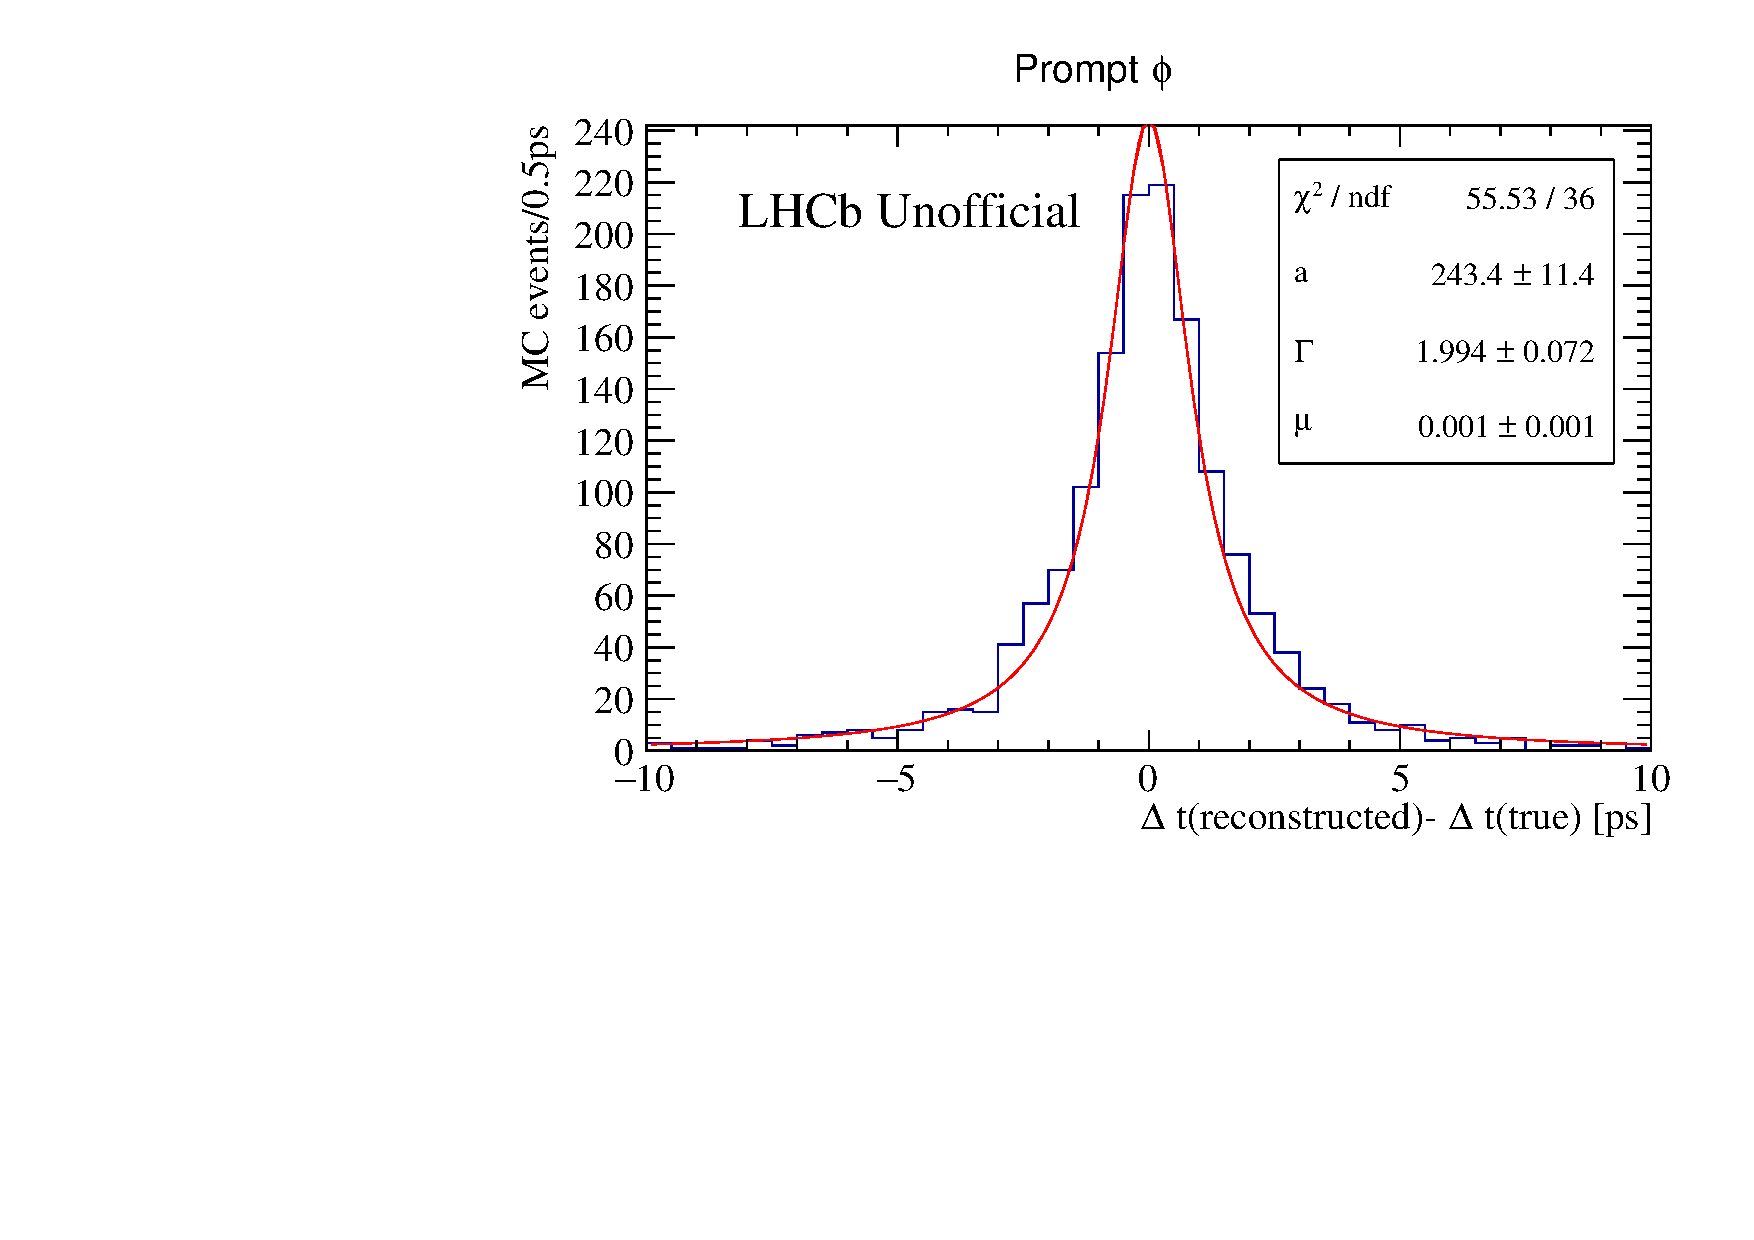
\includegraphics[width=.49\textwidth]{figs/time_res_incl/timeResolution-DeltaTauLL-DTF.pdf}
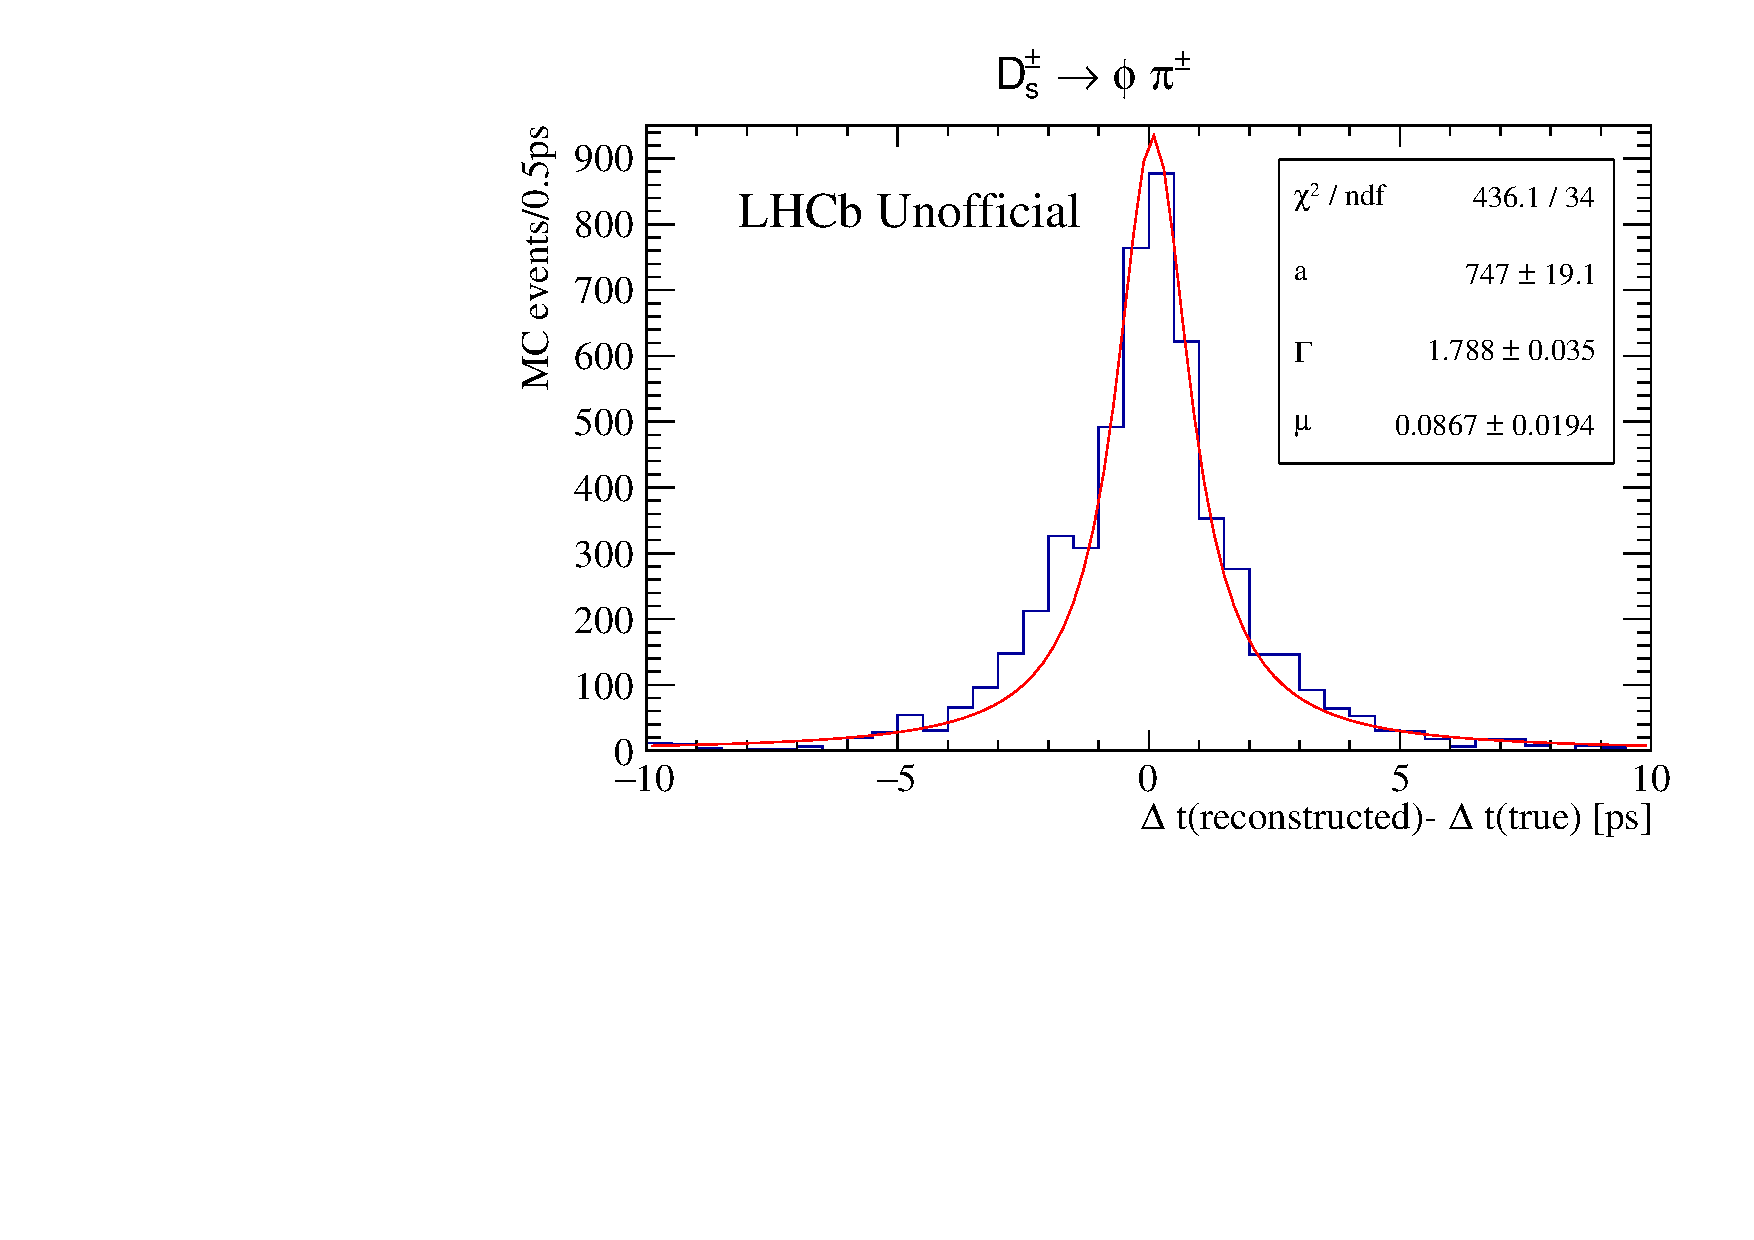
\includegraphics[width=.49\textwidth]{figs/time_res_Ds/timeResolution-DeltaTauLL-DTF.pdf}
\captionof{figure}{Resolution of $\Delta t$ reconstructed via DecayTreeFitter LL kaons. }\label{FIG:timres-LL-DTF-prof}
\end{center}

\begin{center}
\begin{tabular}{c|cc}
Distribution & Prompt $\phi$ & $D_s^\pm \rightarrow \phi \pi^\pm$ \\ 
\hline 
$t$ & $0.127\pm0.006$  & $0.627\pm0.008$ \\ 
$\Delta t$ & $1.99 \pm 0.07$ & $1.79 \pm 0.04$ \\ 
\end{tabular} 
\captionof{table}{Width $\Gamma$ [ps] of the given distributions of decay times and decay time differences for LL kaons reconstructed via the DecayTreeFitter.} \label{TAB:DTF}
\end{center}

\subsection{Using the TupleToolPropertime}
The TupleToolPropertime does not explicitly exclude negative decay times. Therefore, the difference between reconstructed and true decay time relative to the true decay time is symmetric as seen in figures \ref{FIG:LL} and \ref{FIG:DD}. The average residual of the decay time in figure \ref{FIG:all-prof} confirms this.

\begin{center}
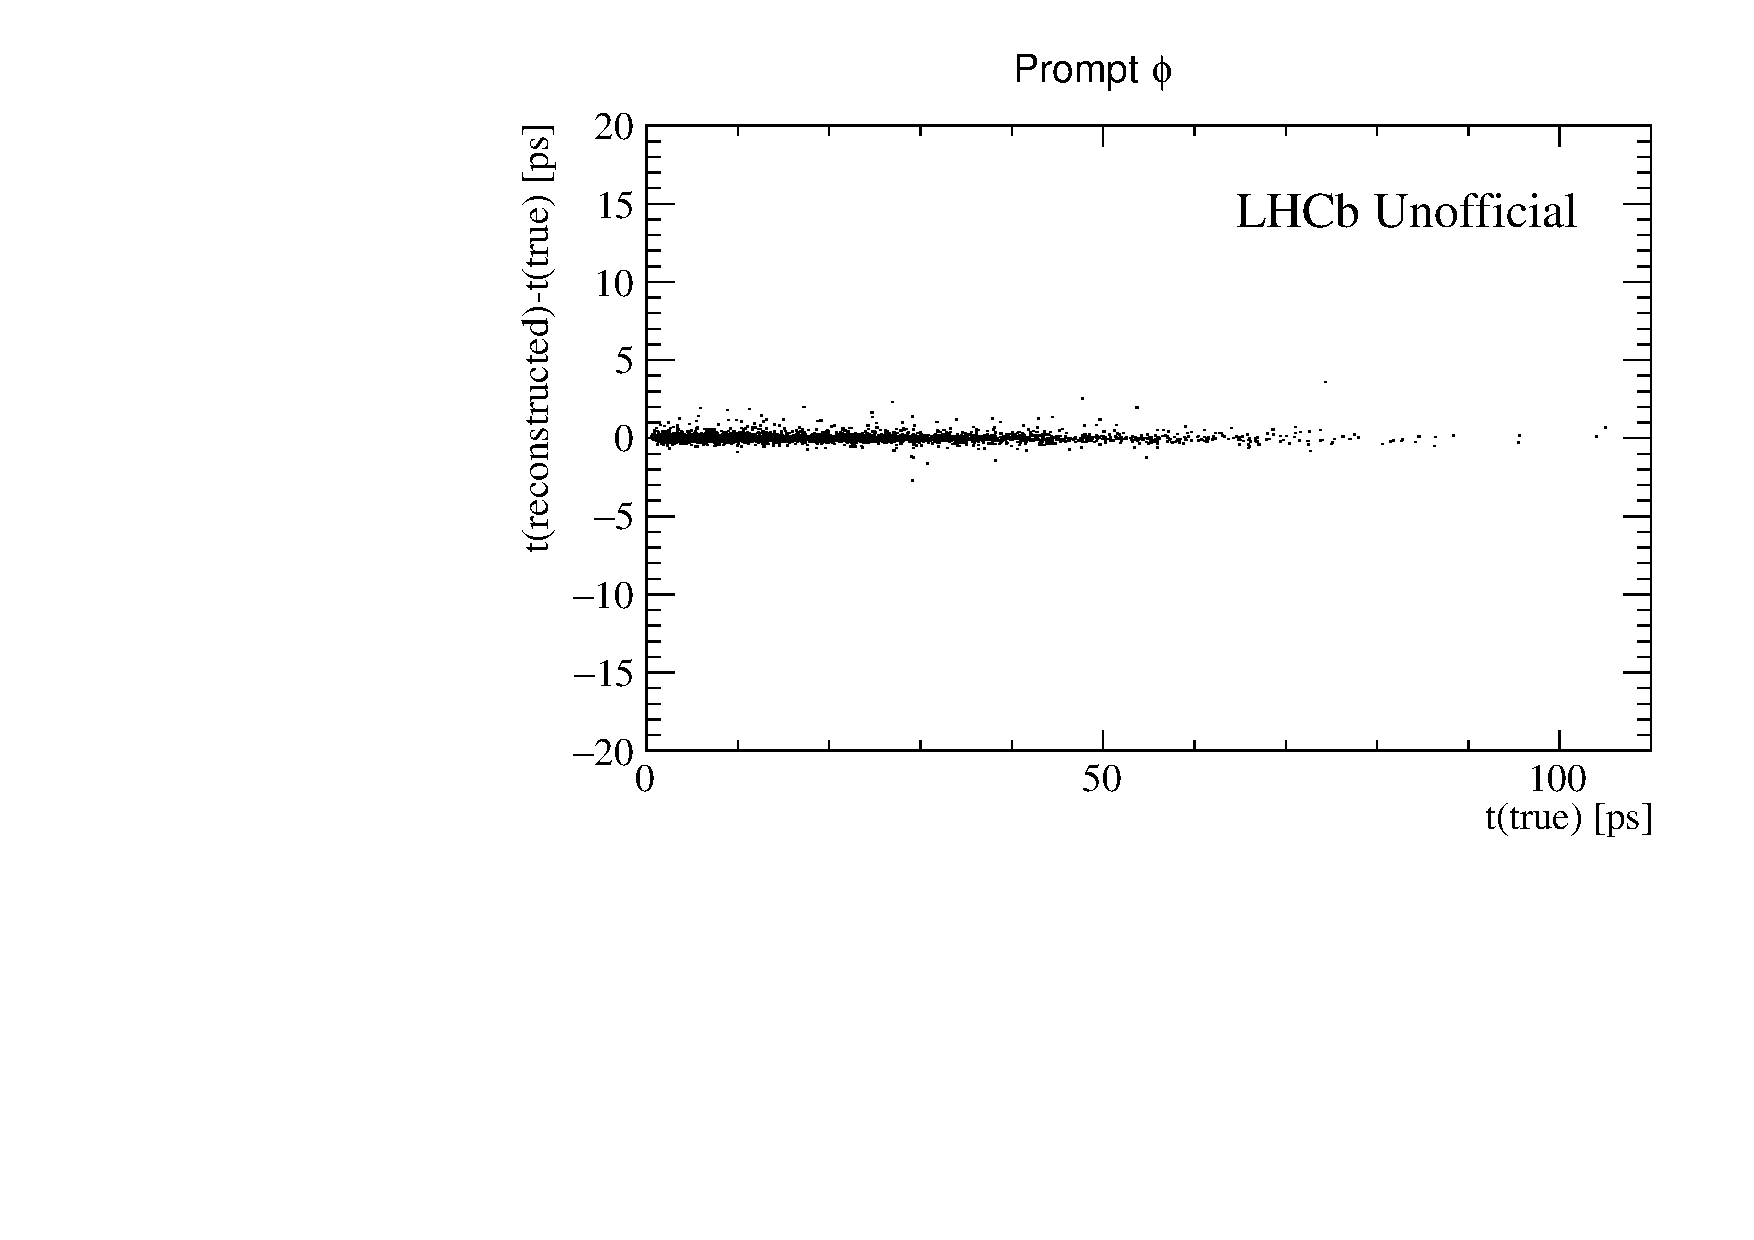
\includegraphics[width=.49\textwidth]{figs/time_res_incl/LL.pdf}
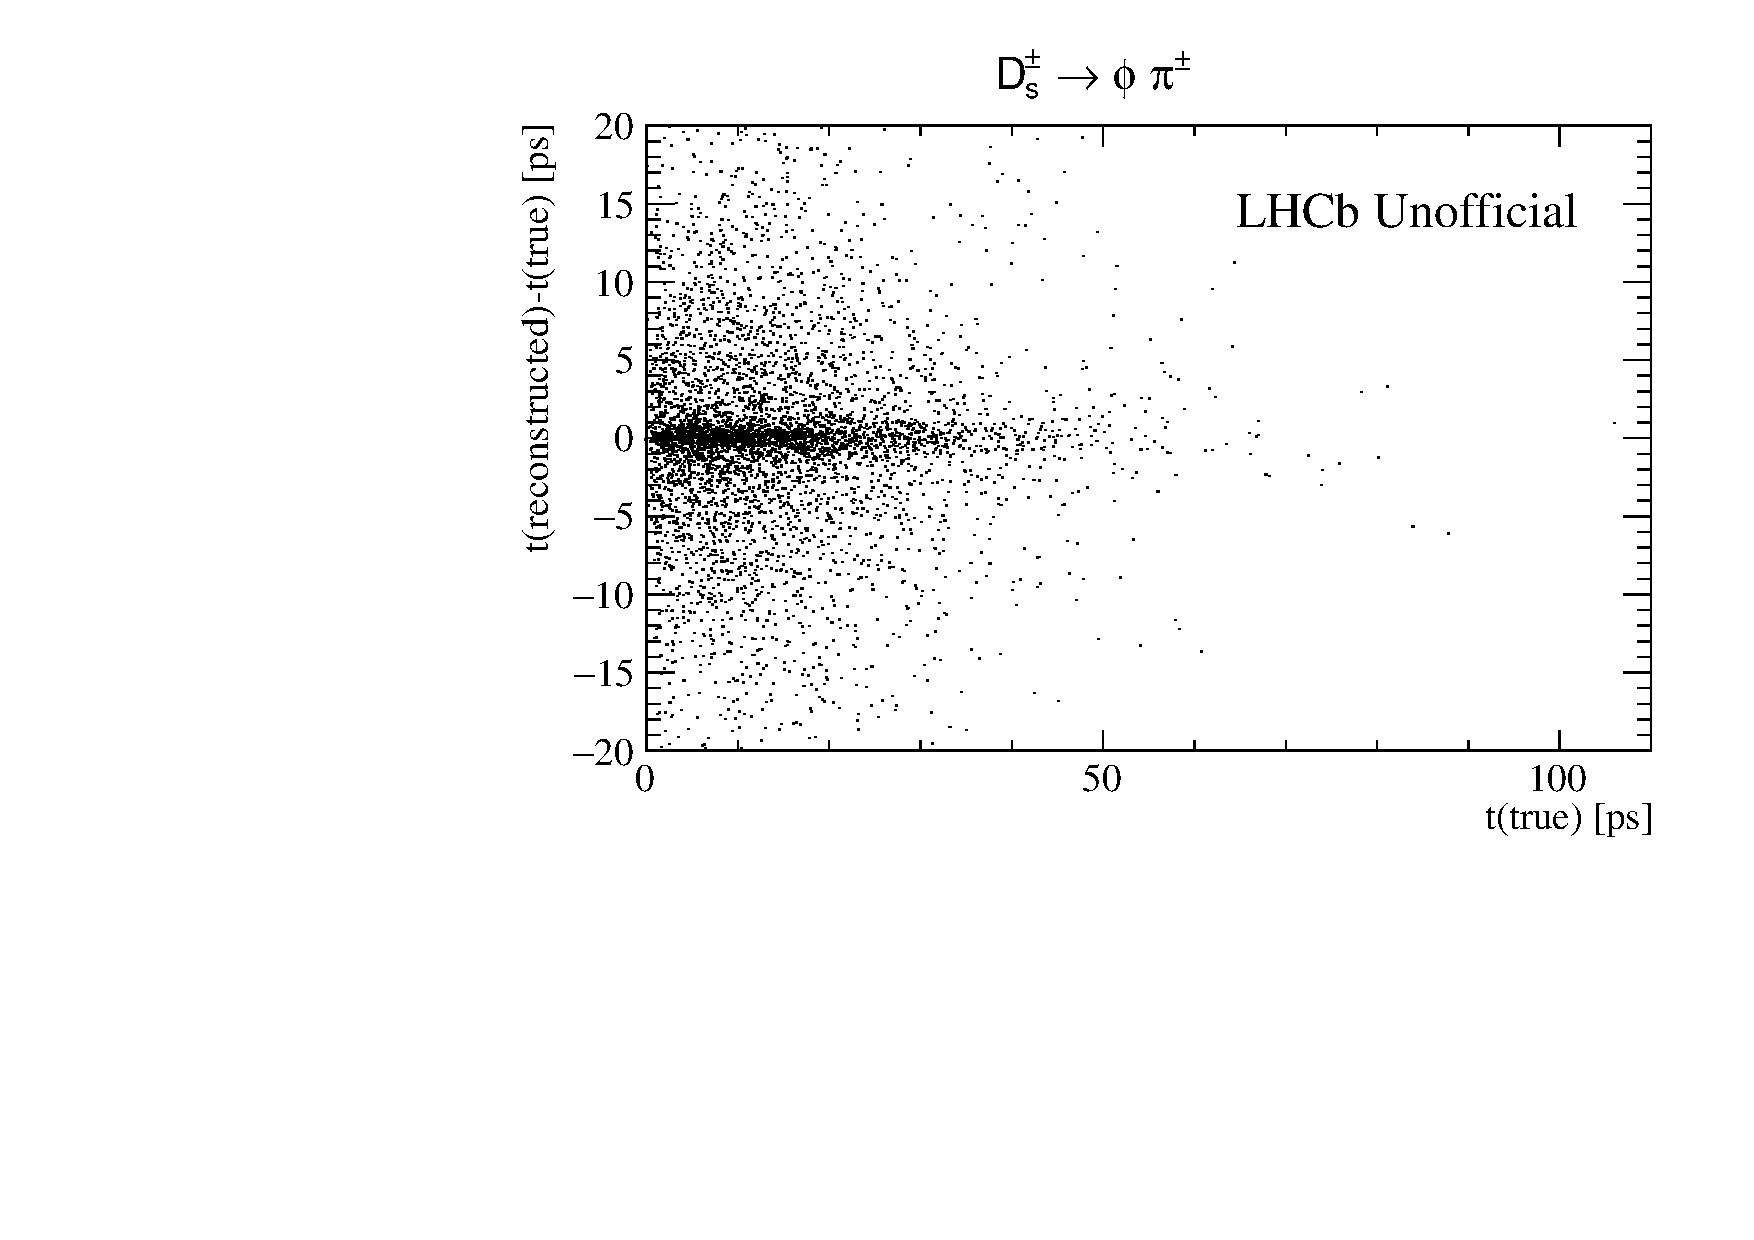
\includegraphics[width=.49\textwidth]{figs/time_res_Ds/LL.pdf}
\captionof{figure}{Residual of $t$ for LL kaons reconstructed using the TupleToolPropertime plotted against the true value of $t$. }\label{FIG:LL}

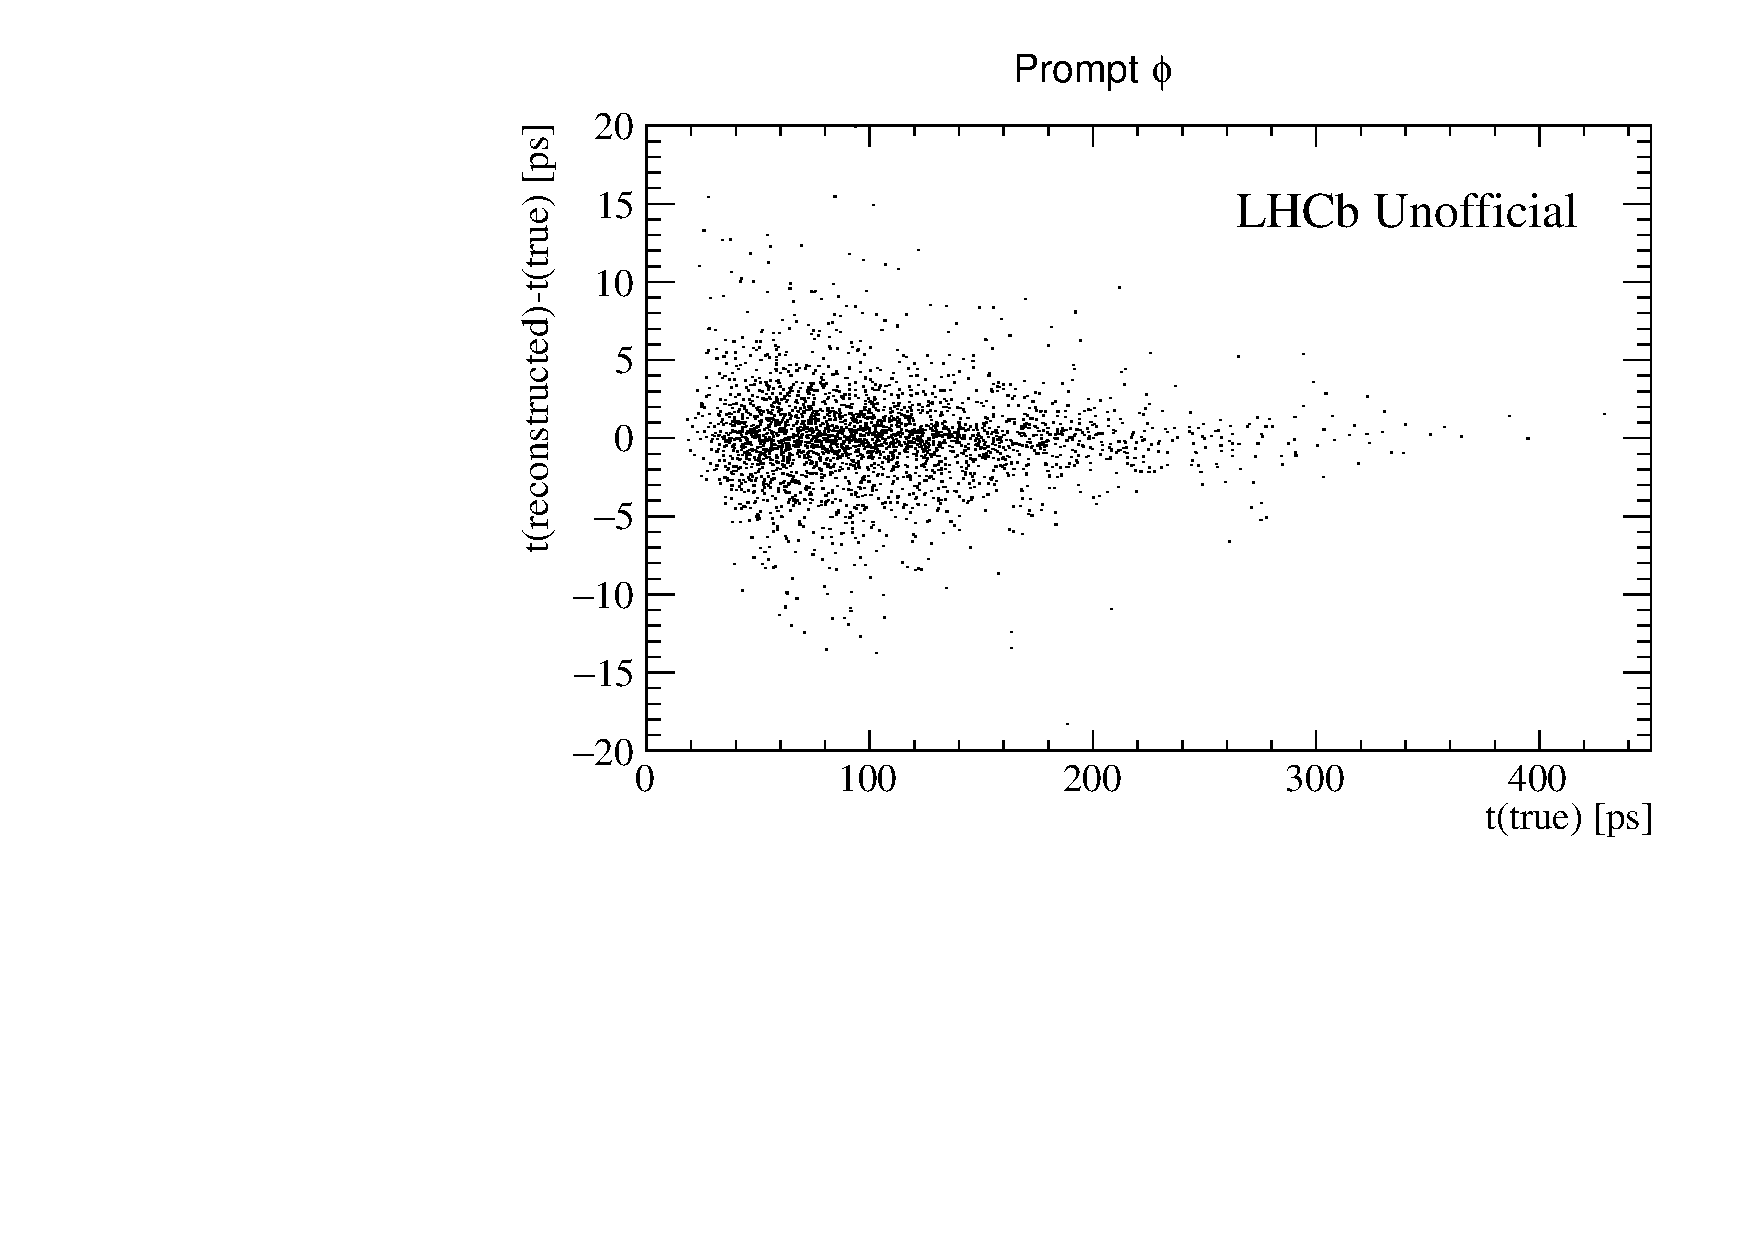
\includegraphics[width=.49\textwidth]{figs/time_res_incl/DD.pdf}
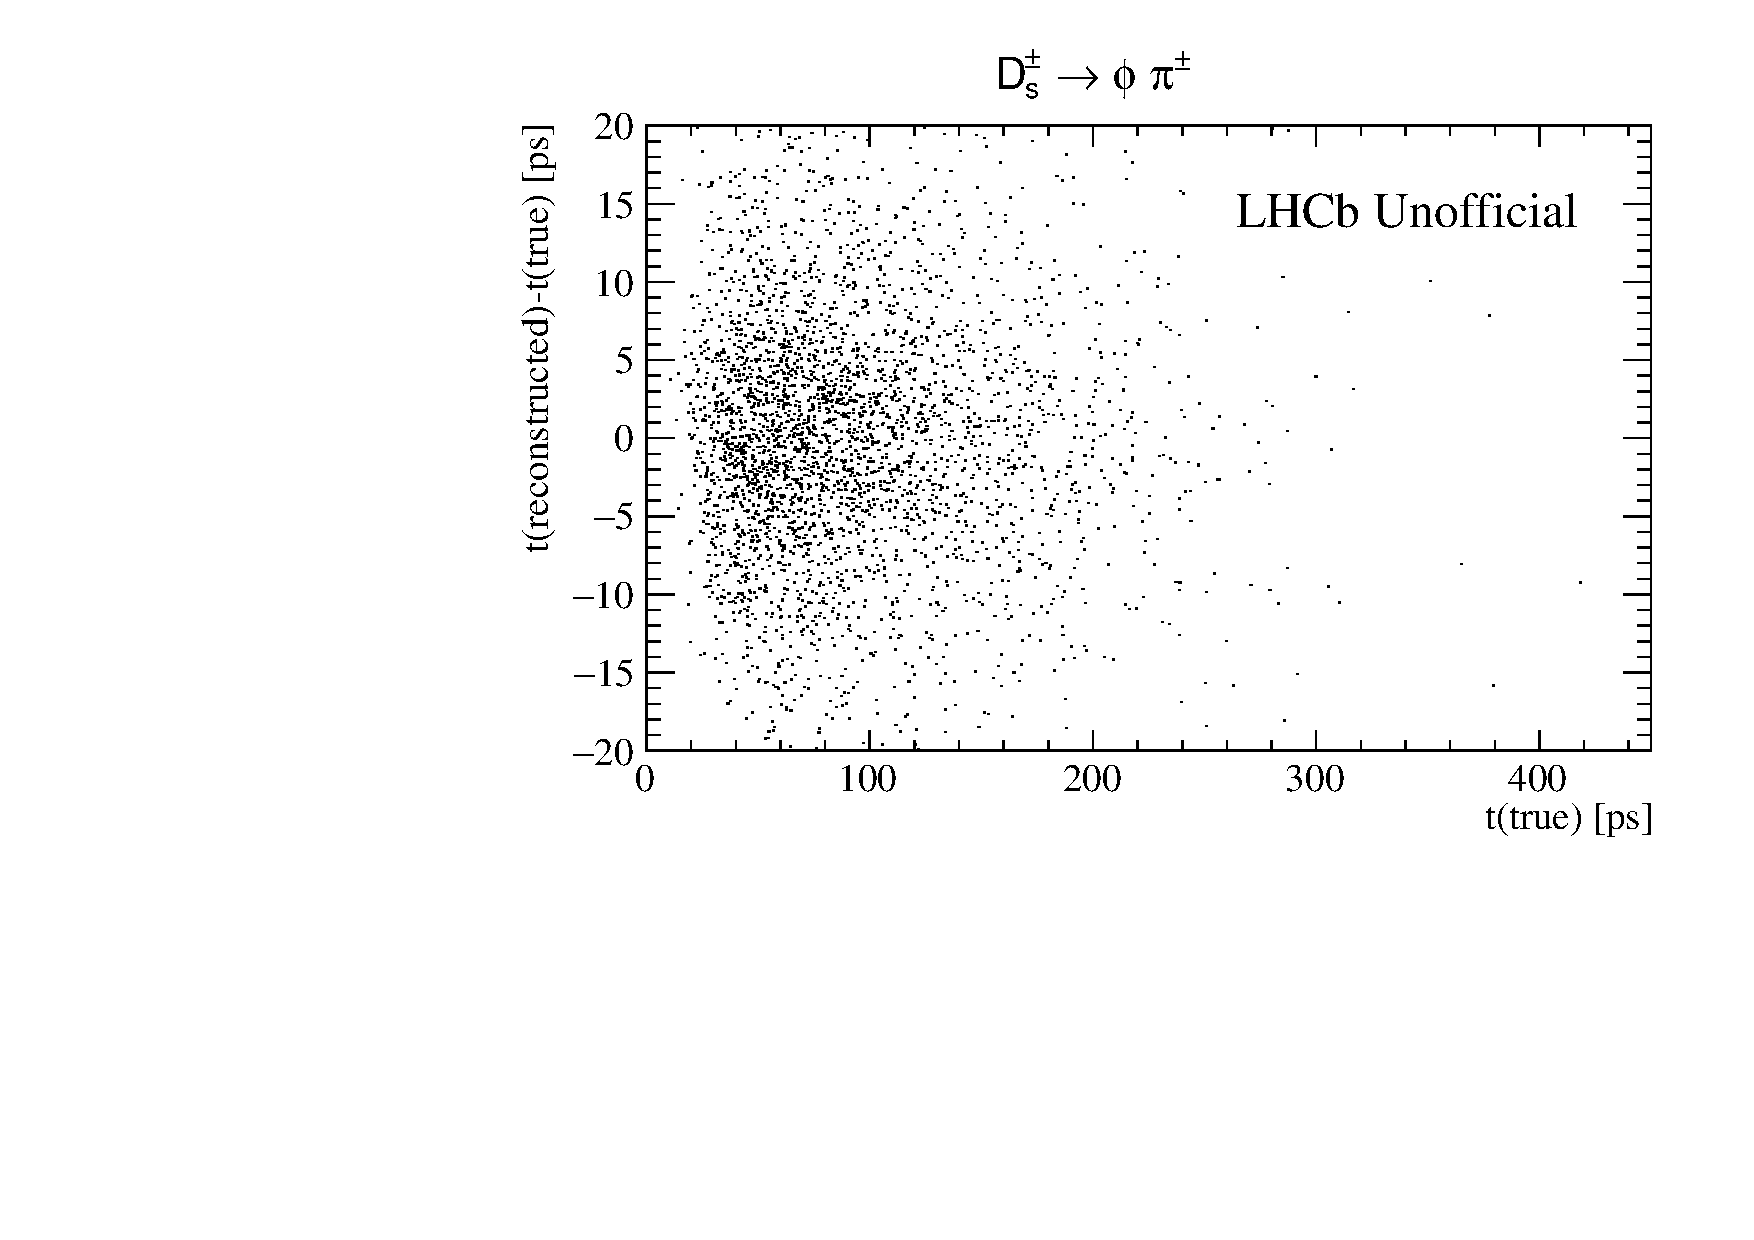
\includegraphics[width=.49\textwidth]{figs/time_res_Ds/DD.pdf}
\captionof{figure}{Residual of $t$ for DD kaons reconstructed using TupleToolPropertime plotted against the true value of $t$.}\label{FIG:DD}
\end{center}


\begin{center}
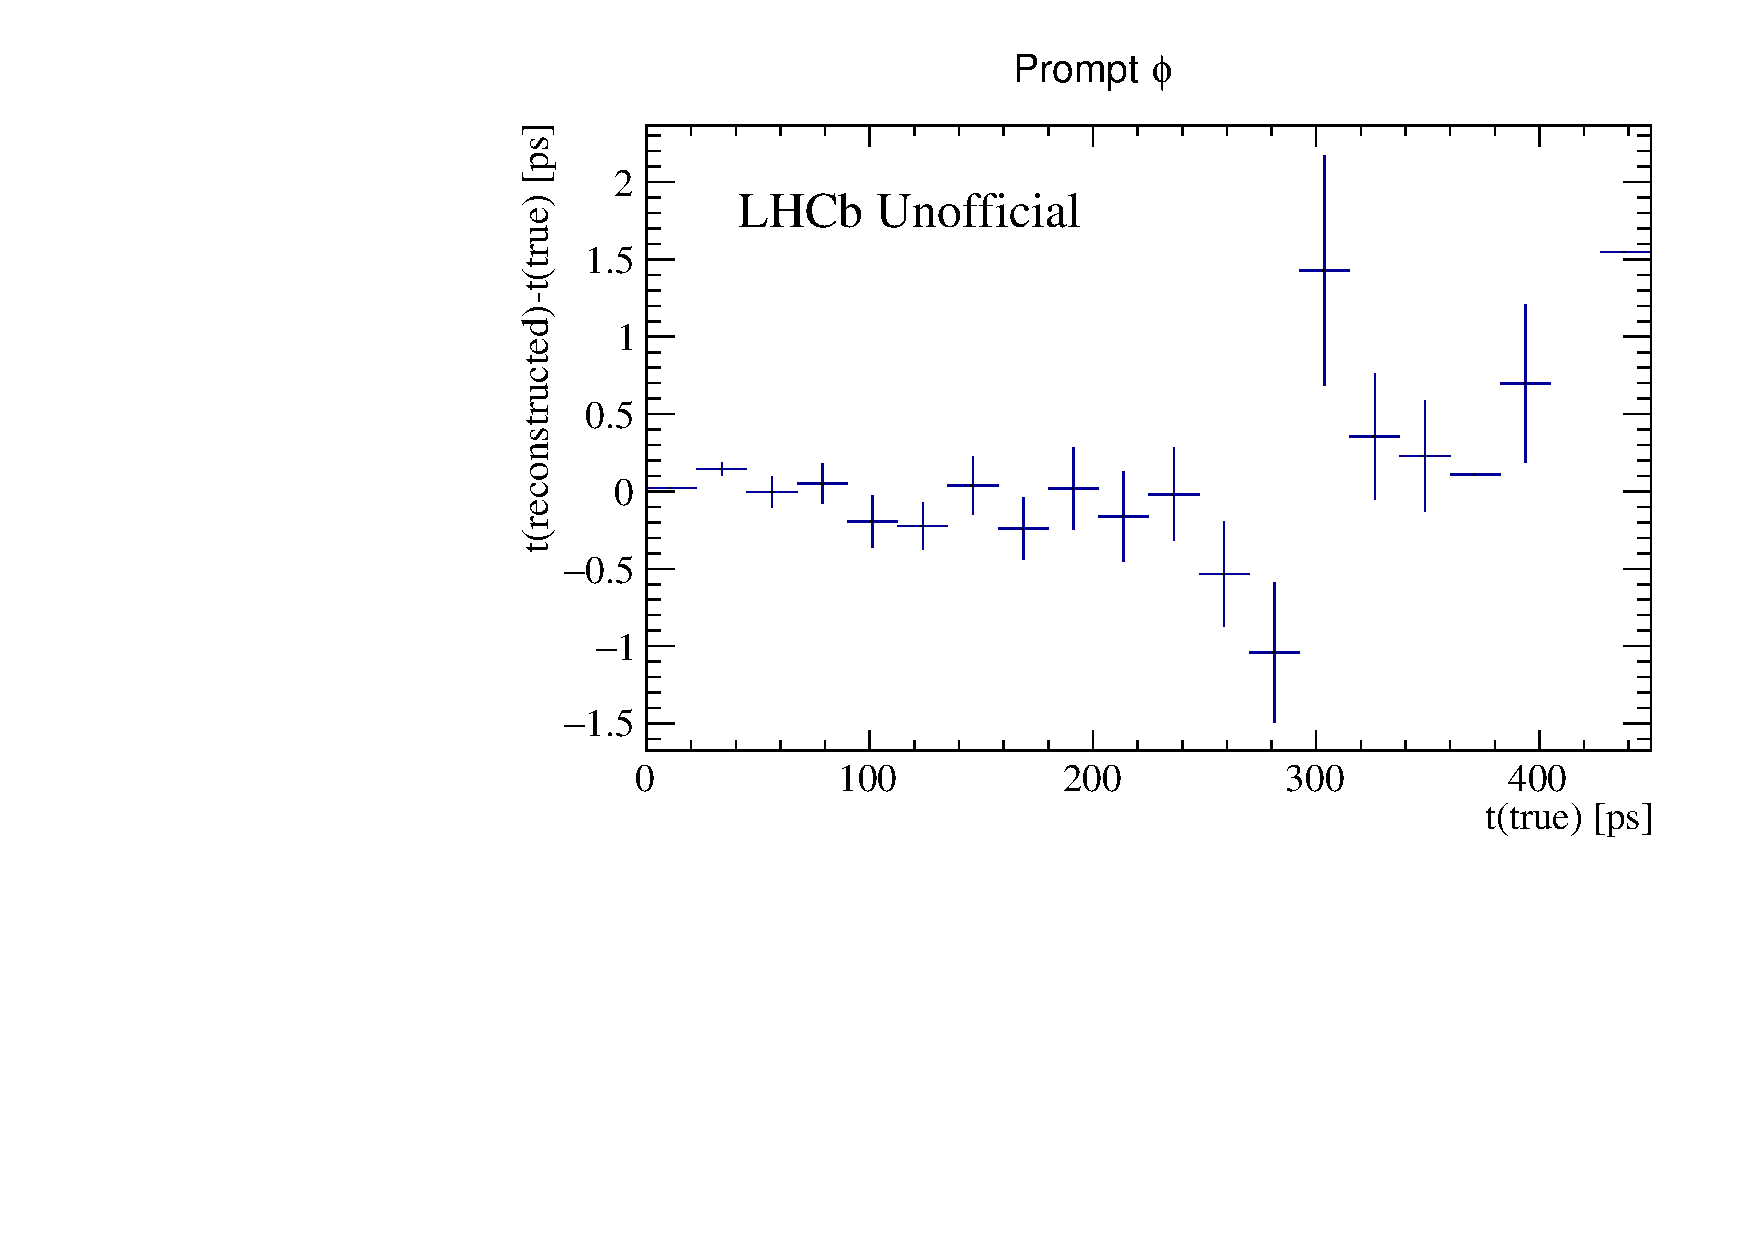
\includegraphics[width=.49\textwidth]{figs/time_res_incl/all-prof.pdf}
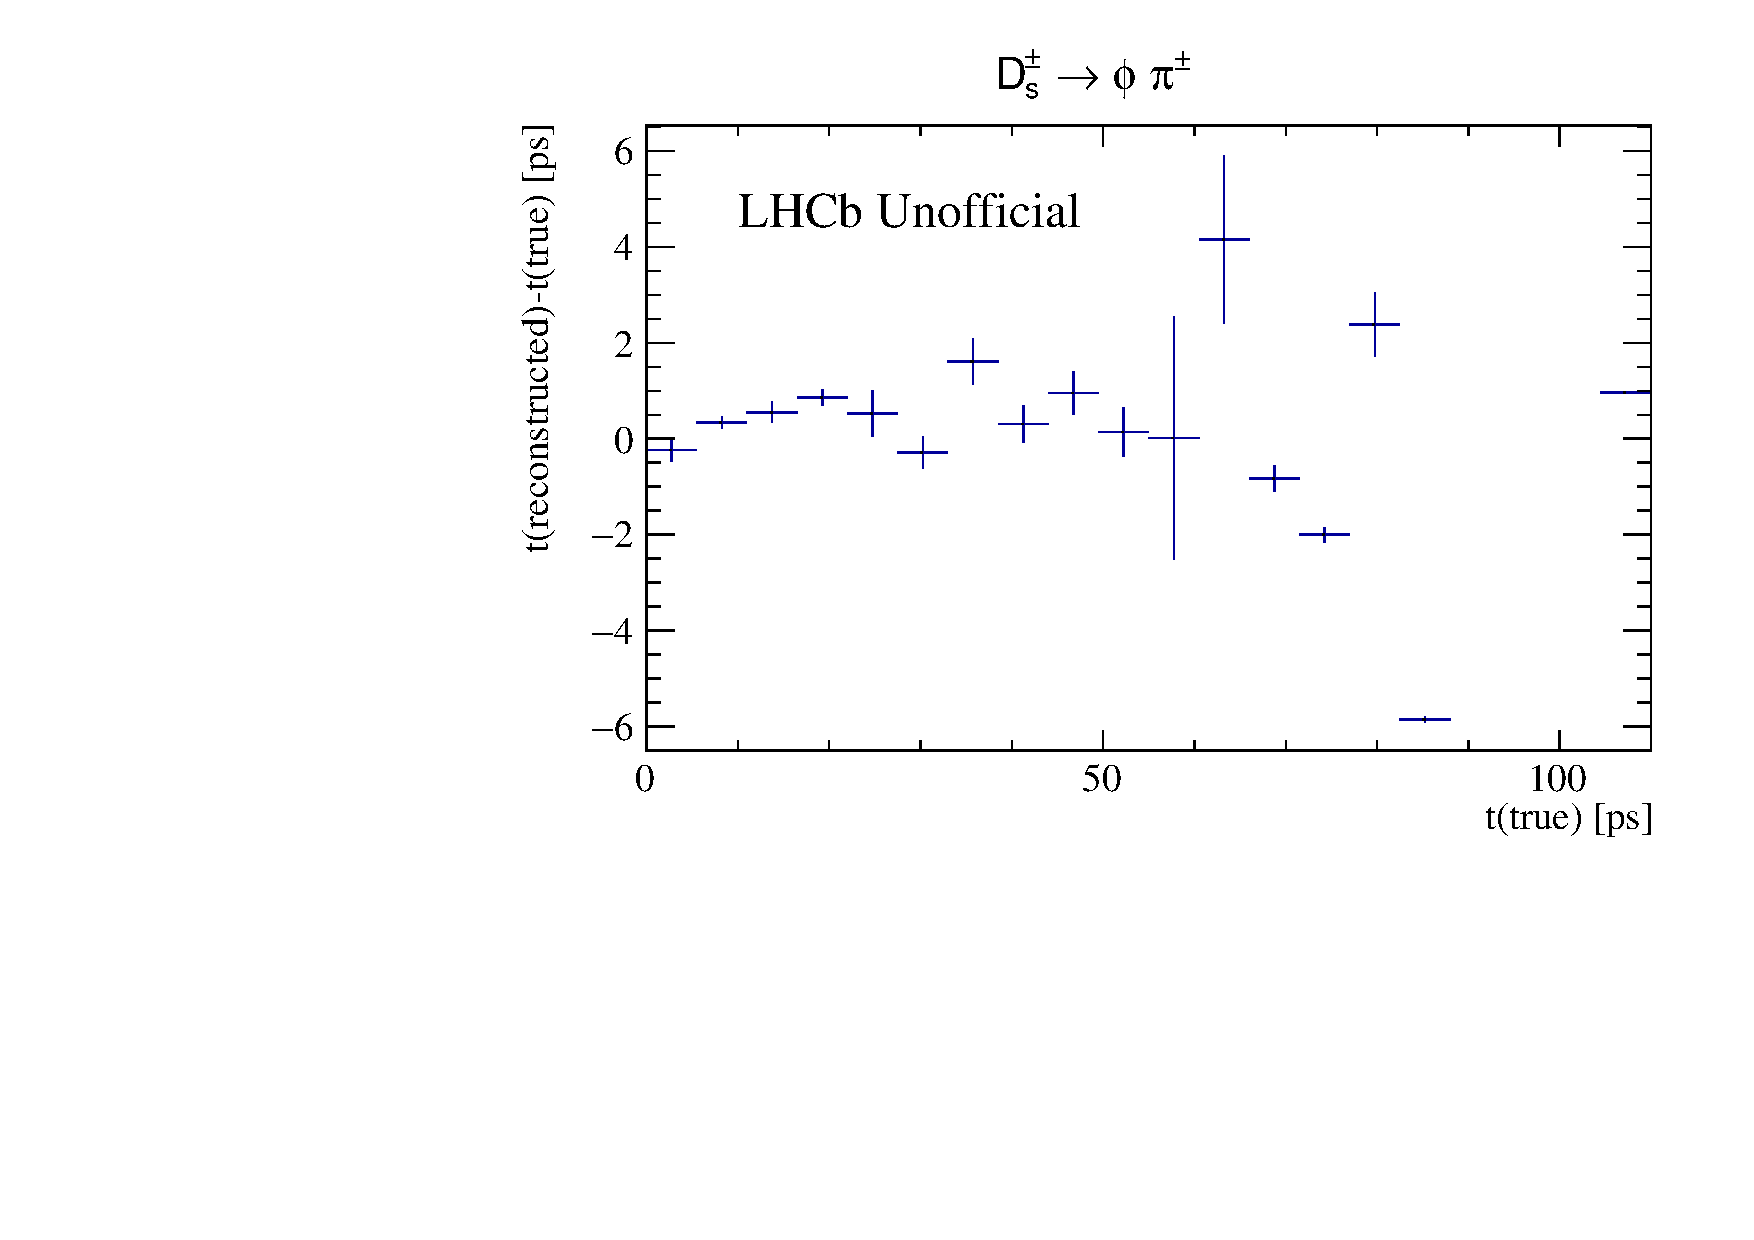
\includegraphics[width=.49\textwidth]{figs/time_res_Ds/LL-prof.pdf}
\captionof{figure}{Average of $t$ reconstructed using TupleToolPropertime for all kaons plotted against the true value of $t$.}\label{FIG:all-prof}
\end{center}
The decay time resolution has been fitted to the Breit Wigner distribution in equation \eqref{EQ:BWt} as shown in figures \ref{FIG:LL-res} and \ref{FIG:DD-res} with the following results for the width:

\begin{center}
\begin{tabular}{c|cc}
& Prompt $\phi$ & $D_s^\pm\rightarrow \phi \pi^\pm$ \\ 
\hline 
LL& $0.126 \pm 0.003$ & $1.55 \pm 0.04$ \\ 
DD& $2.54 \pm 0.07$ & $10.64 \pm 0.14$ \\ 
\end{tabular} 
\captionof{table}{Width $\Gamma$ [ps] of the time resolution for the reconstruction with TupleToolPropertime.}
\end{center}

\begin{center}
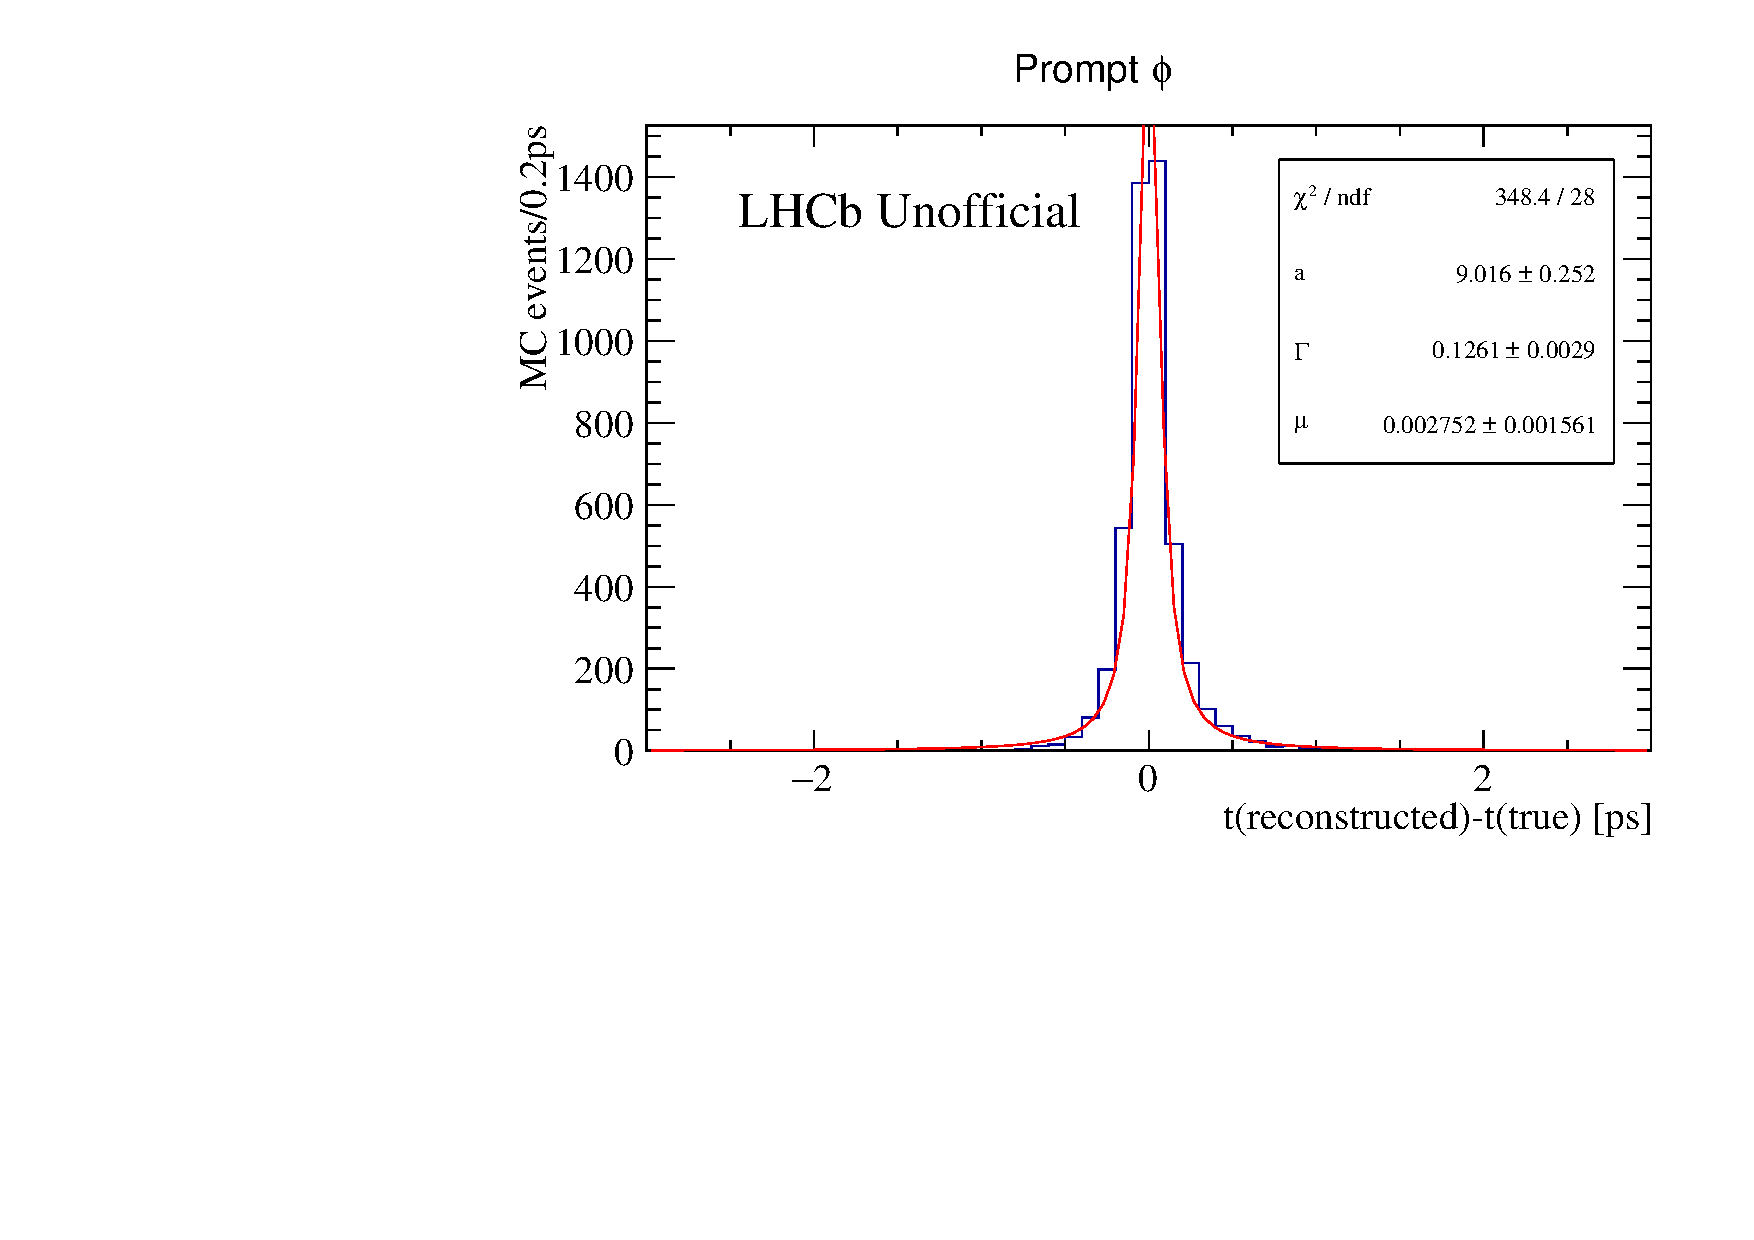
\includegraphics[width=.49\textwidth]{figs/time_res_incl/timeResolution-LL.pdf}
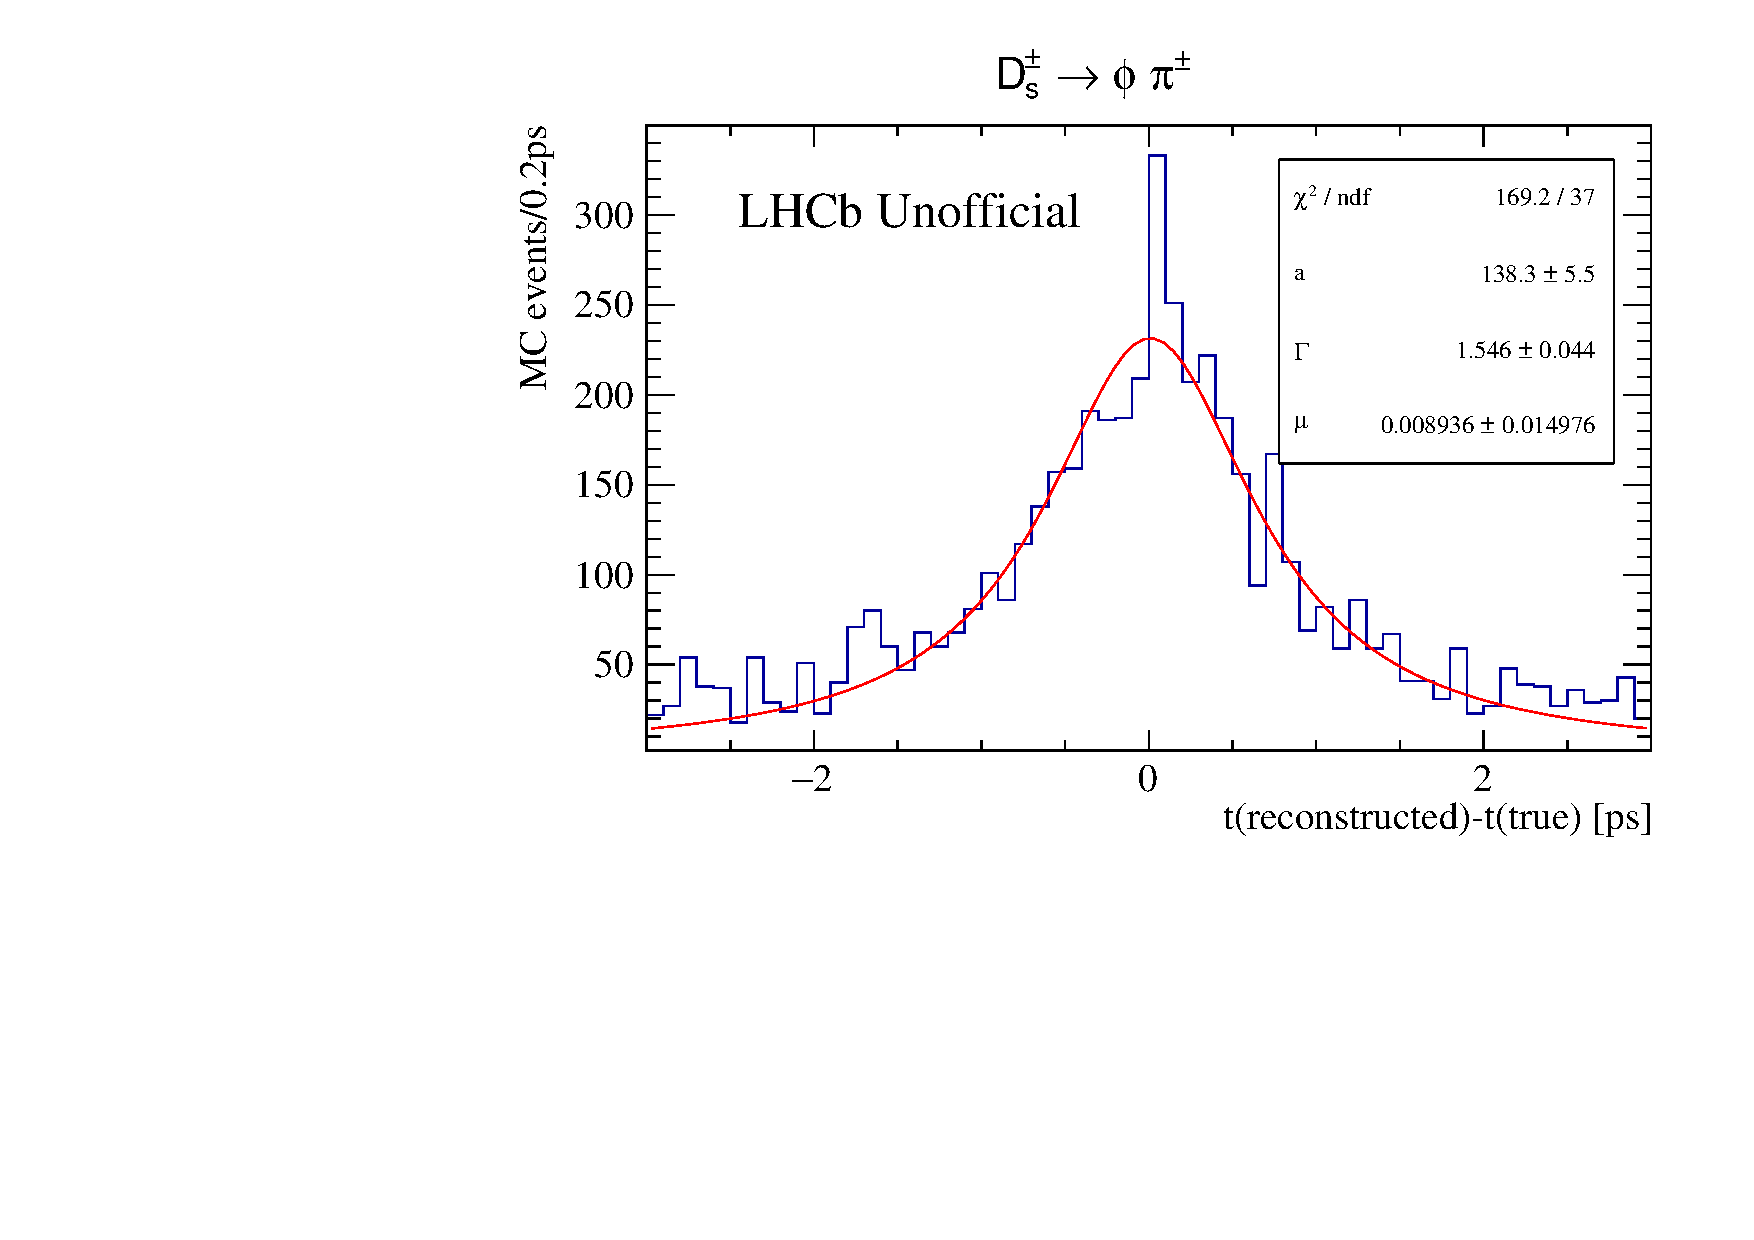
\includegraphics[width=.49\textwidth]{figs/time_res_Ds/timeResolution-LL.pdf}
\captionof{figure}{Resolution of LL kaon decay times $t$ reconstructed via the DecayTreeFitter. }\label{FIG:LL-res}


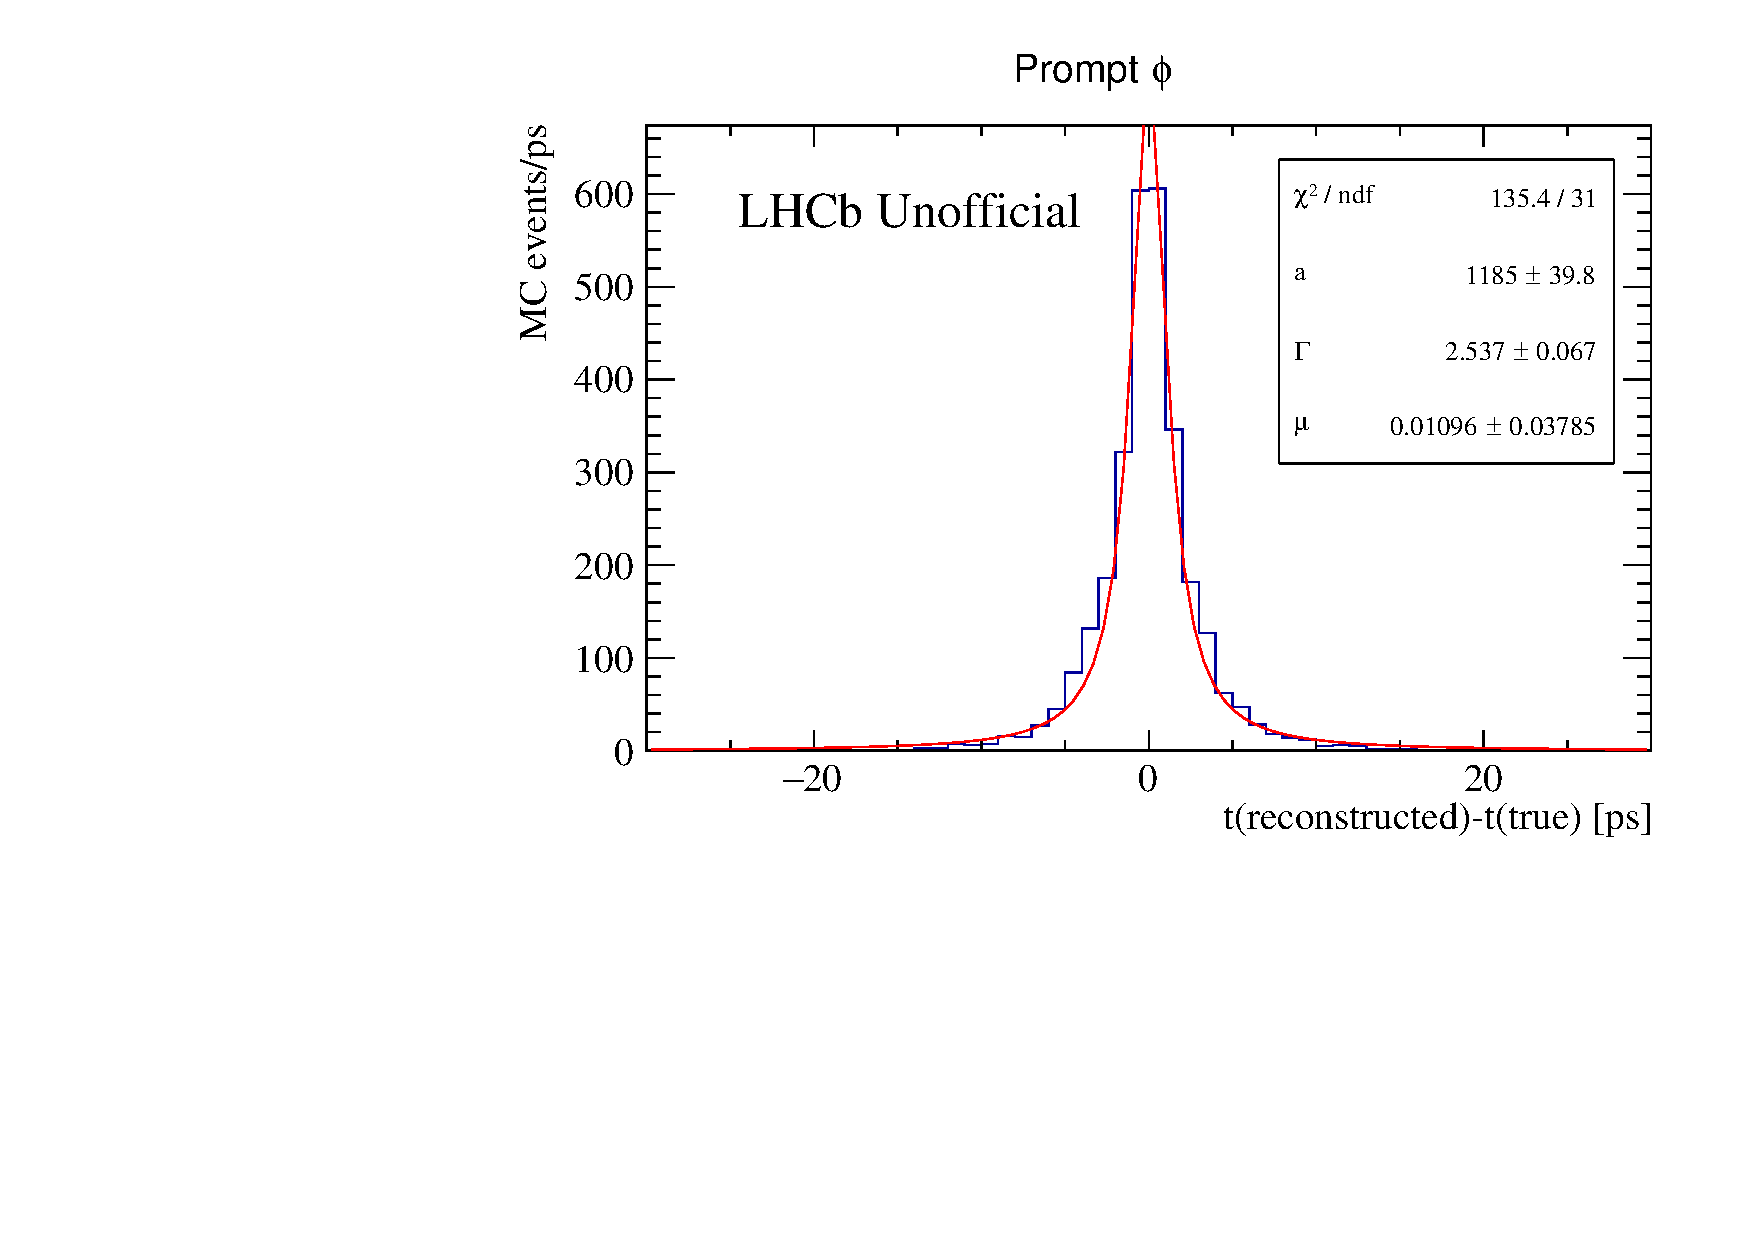
\includegraphics[width=.49\textwidth]{figs/time_res_incl/timeResolution-DD.pdf}
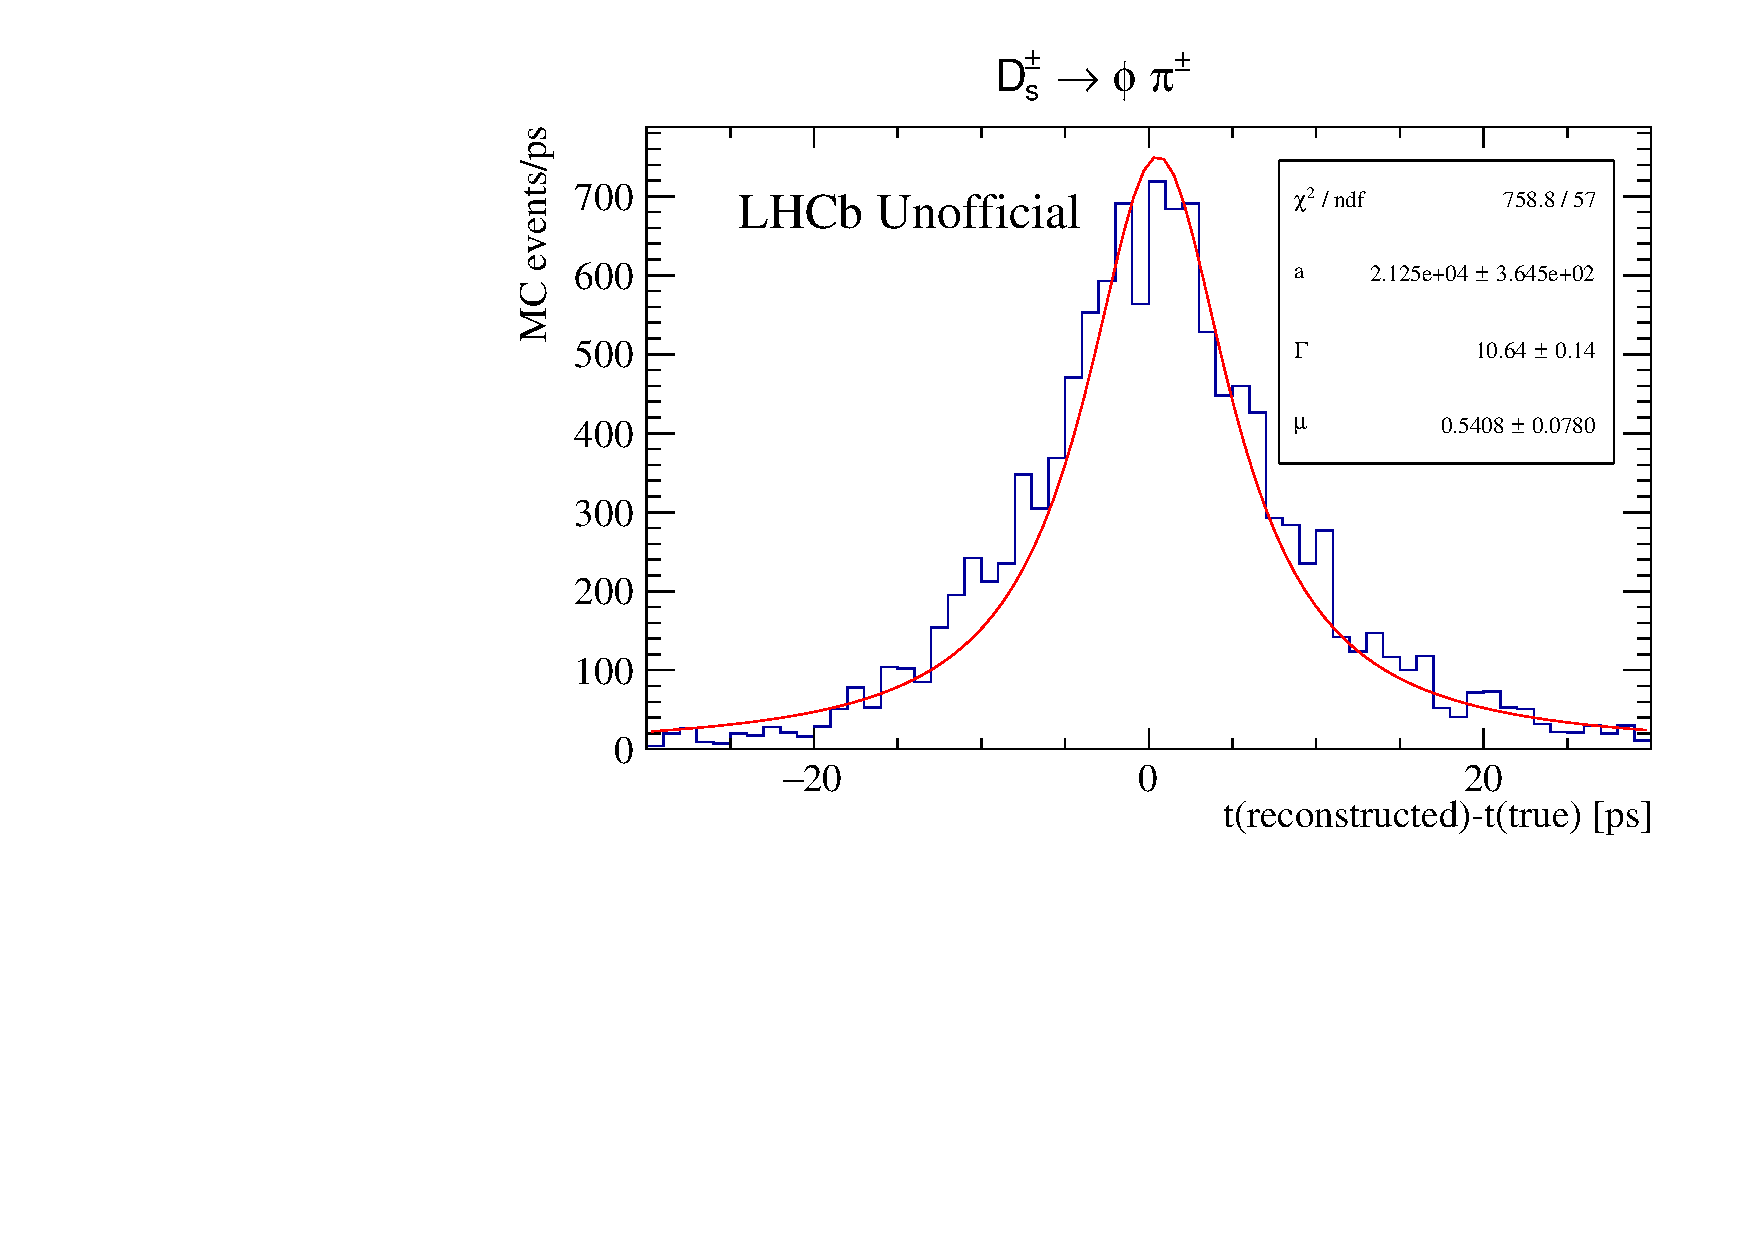
\includegraphics[width=.49\textwidth]{figs/time_res_Ds/timeResolution-DD.pdf}
\captionof{figure}{Resolution of DD kaon decay times $t$ reconstructed via the DecayTreeFitter.  }\label{FIG:DD-res}
\end{center}

Additionally, the resolution of $\Delta t$ has been determined by fitting the Breit Wigner distribution in equation \eqref{EQ:BWdeltat} to the distribution of the residuals. Since in the Monte Carlo either both kaons are LL or one is LL and the other is DD, here, these two combinations have been studied. The plots illustrating the fit can be found in figures \ref{FIG:LL-diff} and \ref{FIG:LD-diff} and the widths in table \ref{TAB:whatever}.



\begin{center}
\begin{tabular}{c|cc}
 & Prompt $\phi$ & $D_s^\pm \rightarrow \phi \pi^\pm$ \\ 
\hline 
LL and LL & $0.24 \pm 0.01$ & $0.43 \pm 0.01$ \\ 
LL and DD & $2.47 \pm 0.06$ & $4.11 \pm 0.05$ \\ 
\end{tabular} 
\captionof{table}{Width $\Gamma$ [ps] of the  decay time differences for kaons reconstructed using the TupleToolPropertime.} \label{TAB:whatever}
\end{center}


\begin{center}
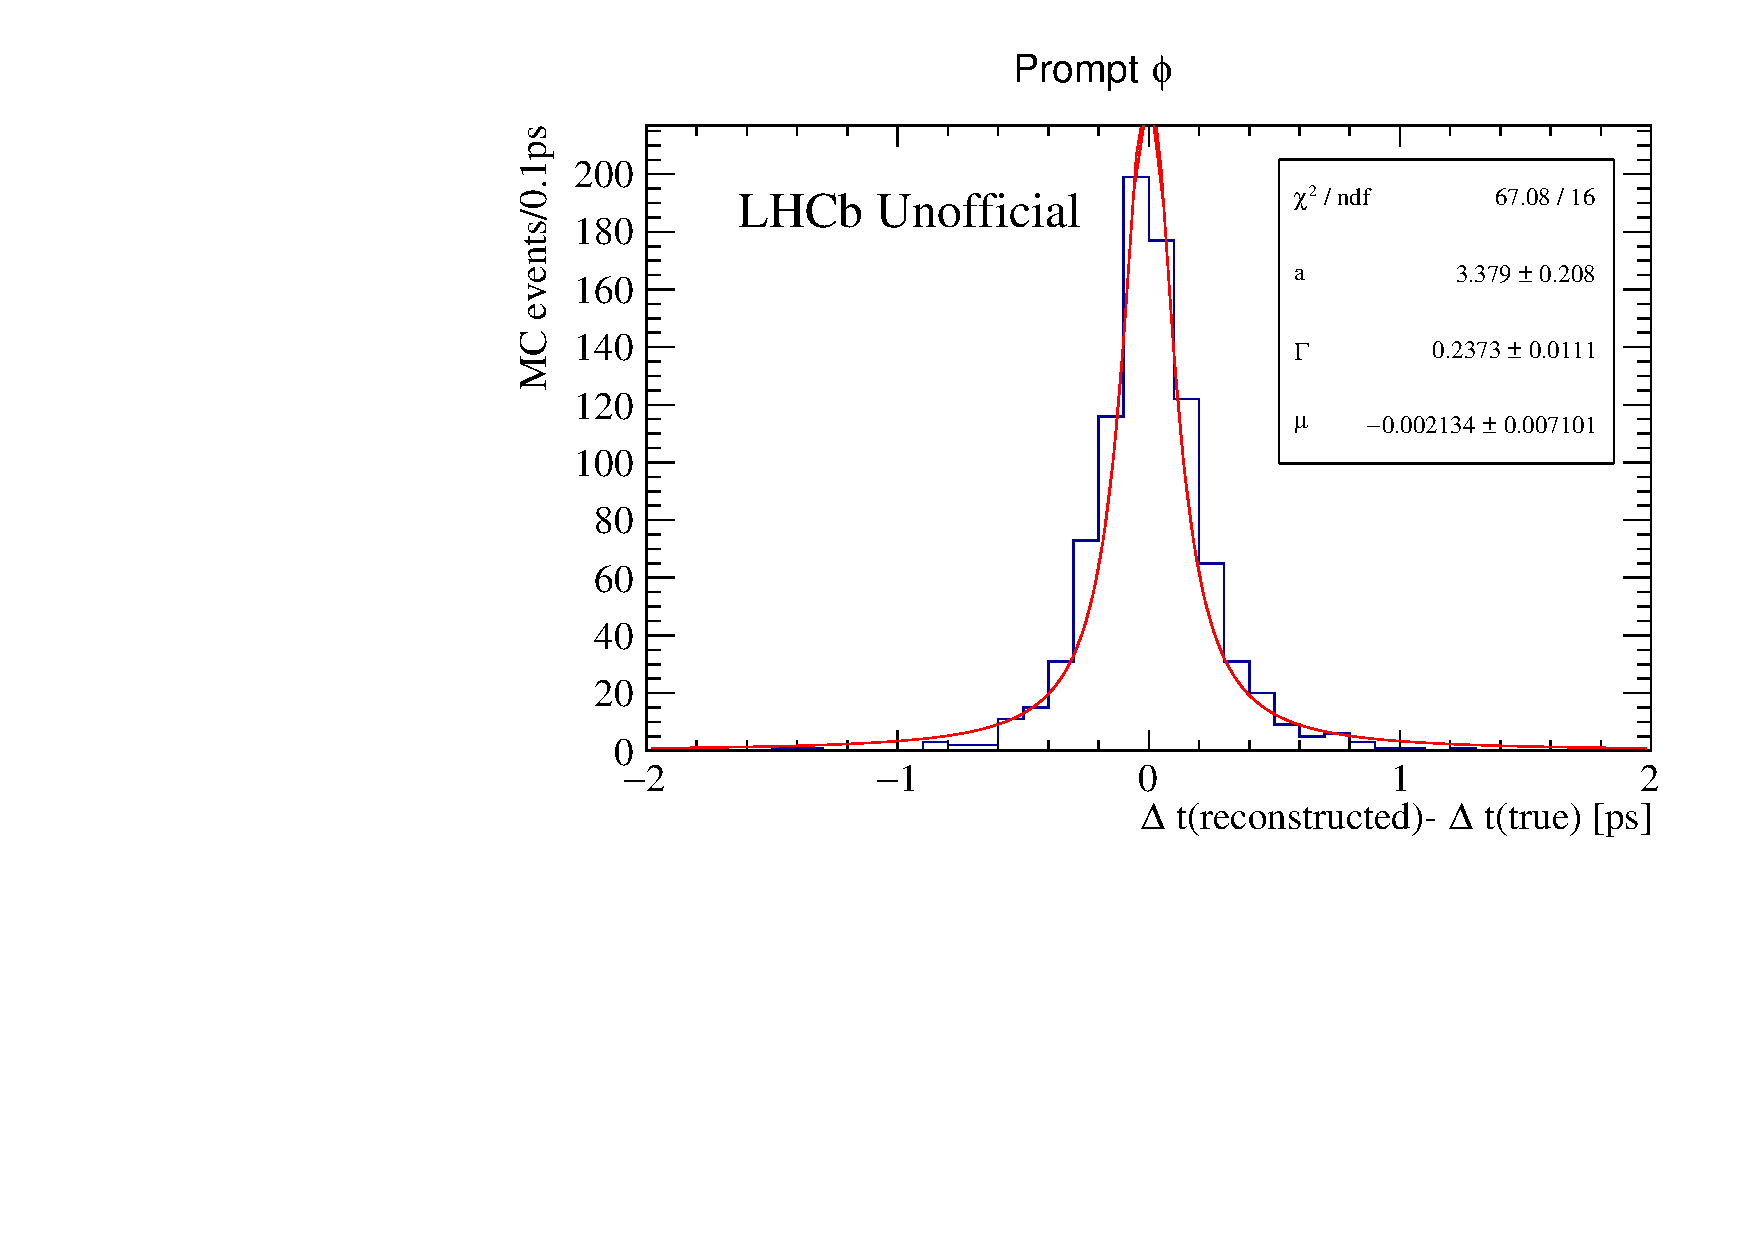
\includegraphics[width=.49\textwidth]{figs/time_res_incl/timeResolution-DeltaTauLL.pdf}
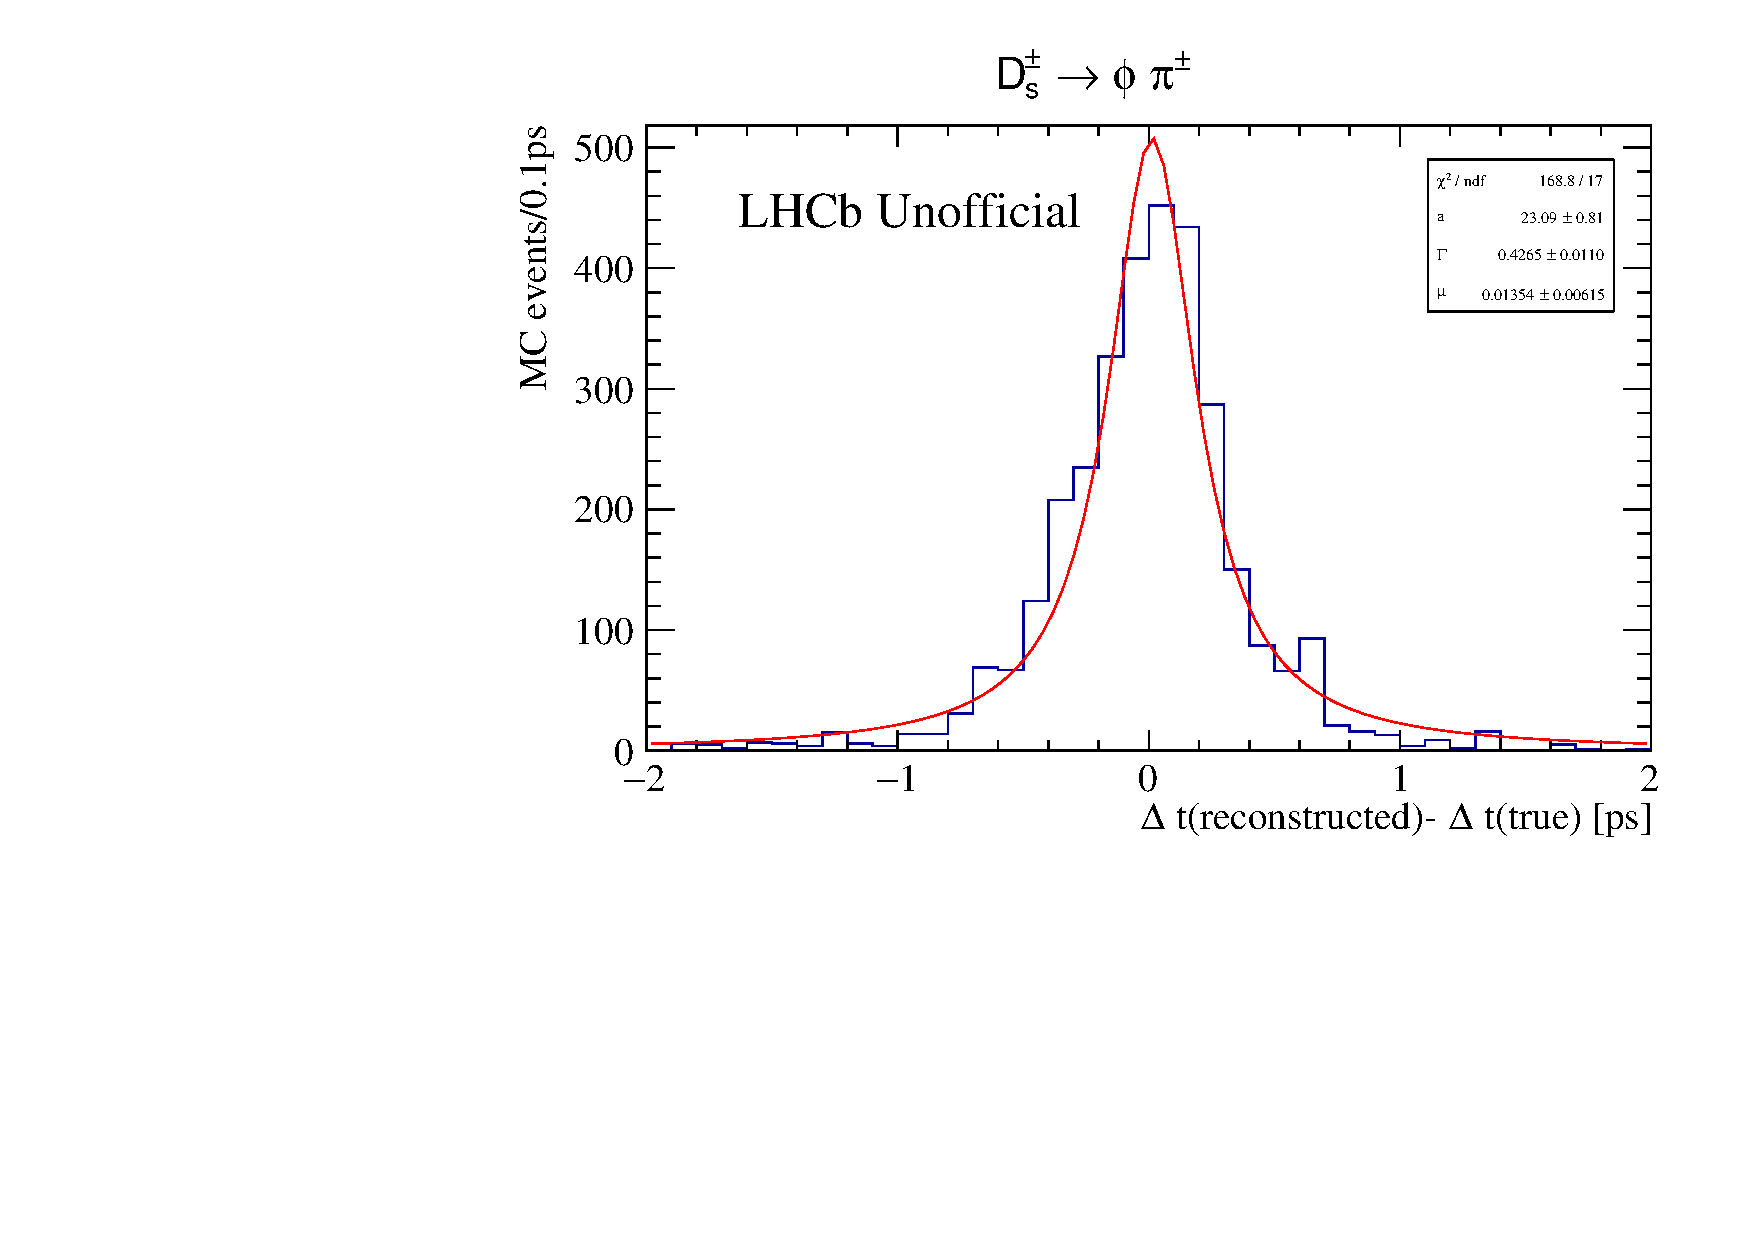
\includegraphics[width=.49\textwidth]{figs/time_res_Ds/timeResolution-DeltaTauLL.pdf}
\captionof{figure}{Resolution of $\Delta t$ for LL kaons reconstructed using the TupleToolPropertime. }\label{FIG:LL-diff}
\end{center}


\begin{center}
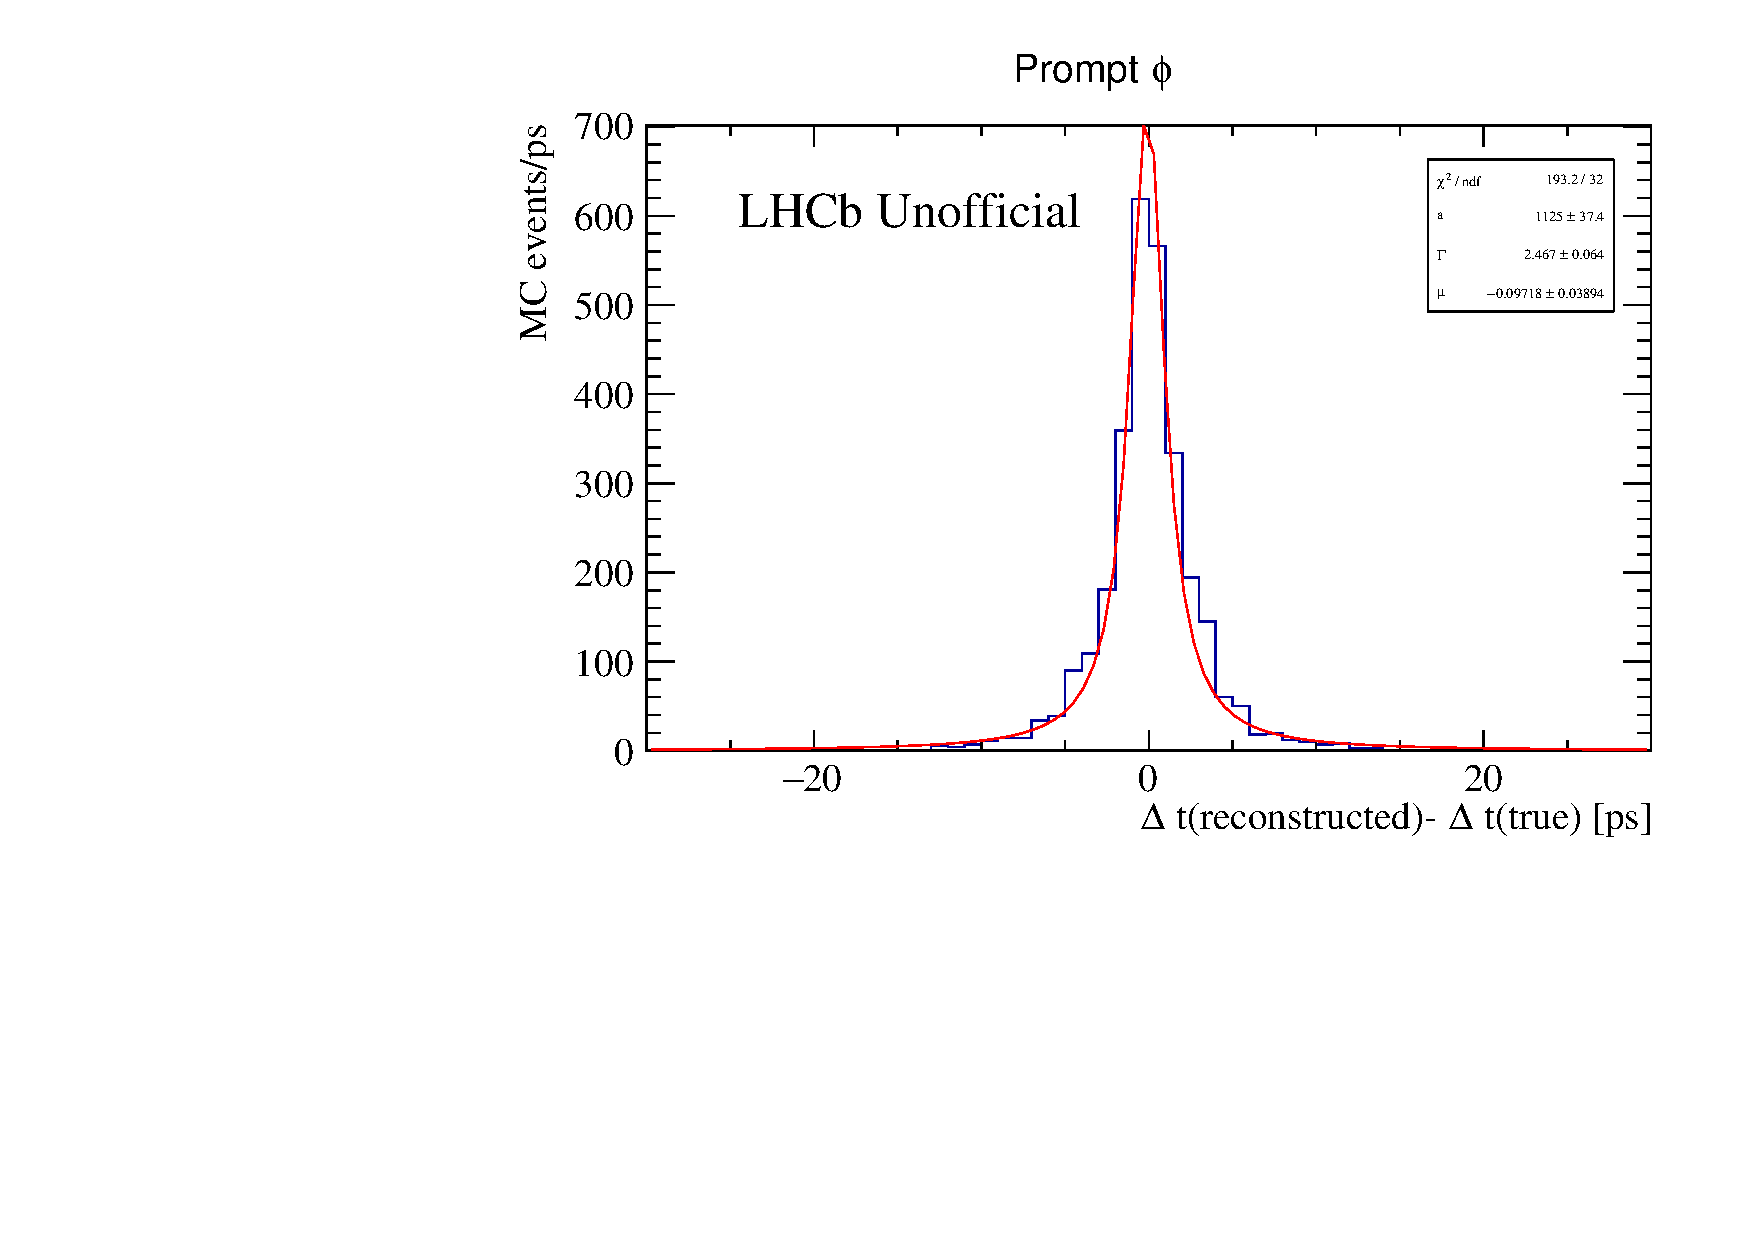
\includegraphics[width=.49\textwidth]{figs/time_res_incl/timeResolution-DeltaTauLD.pdf}
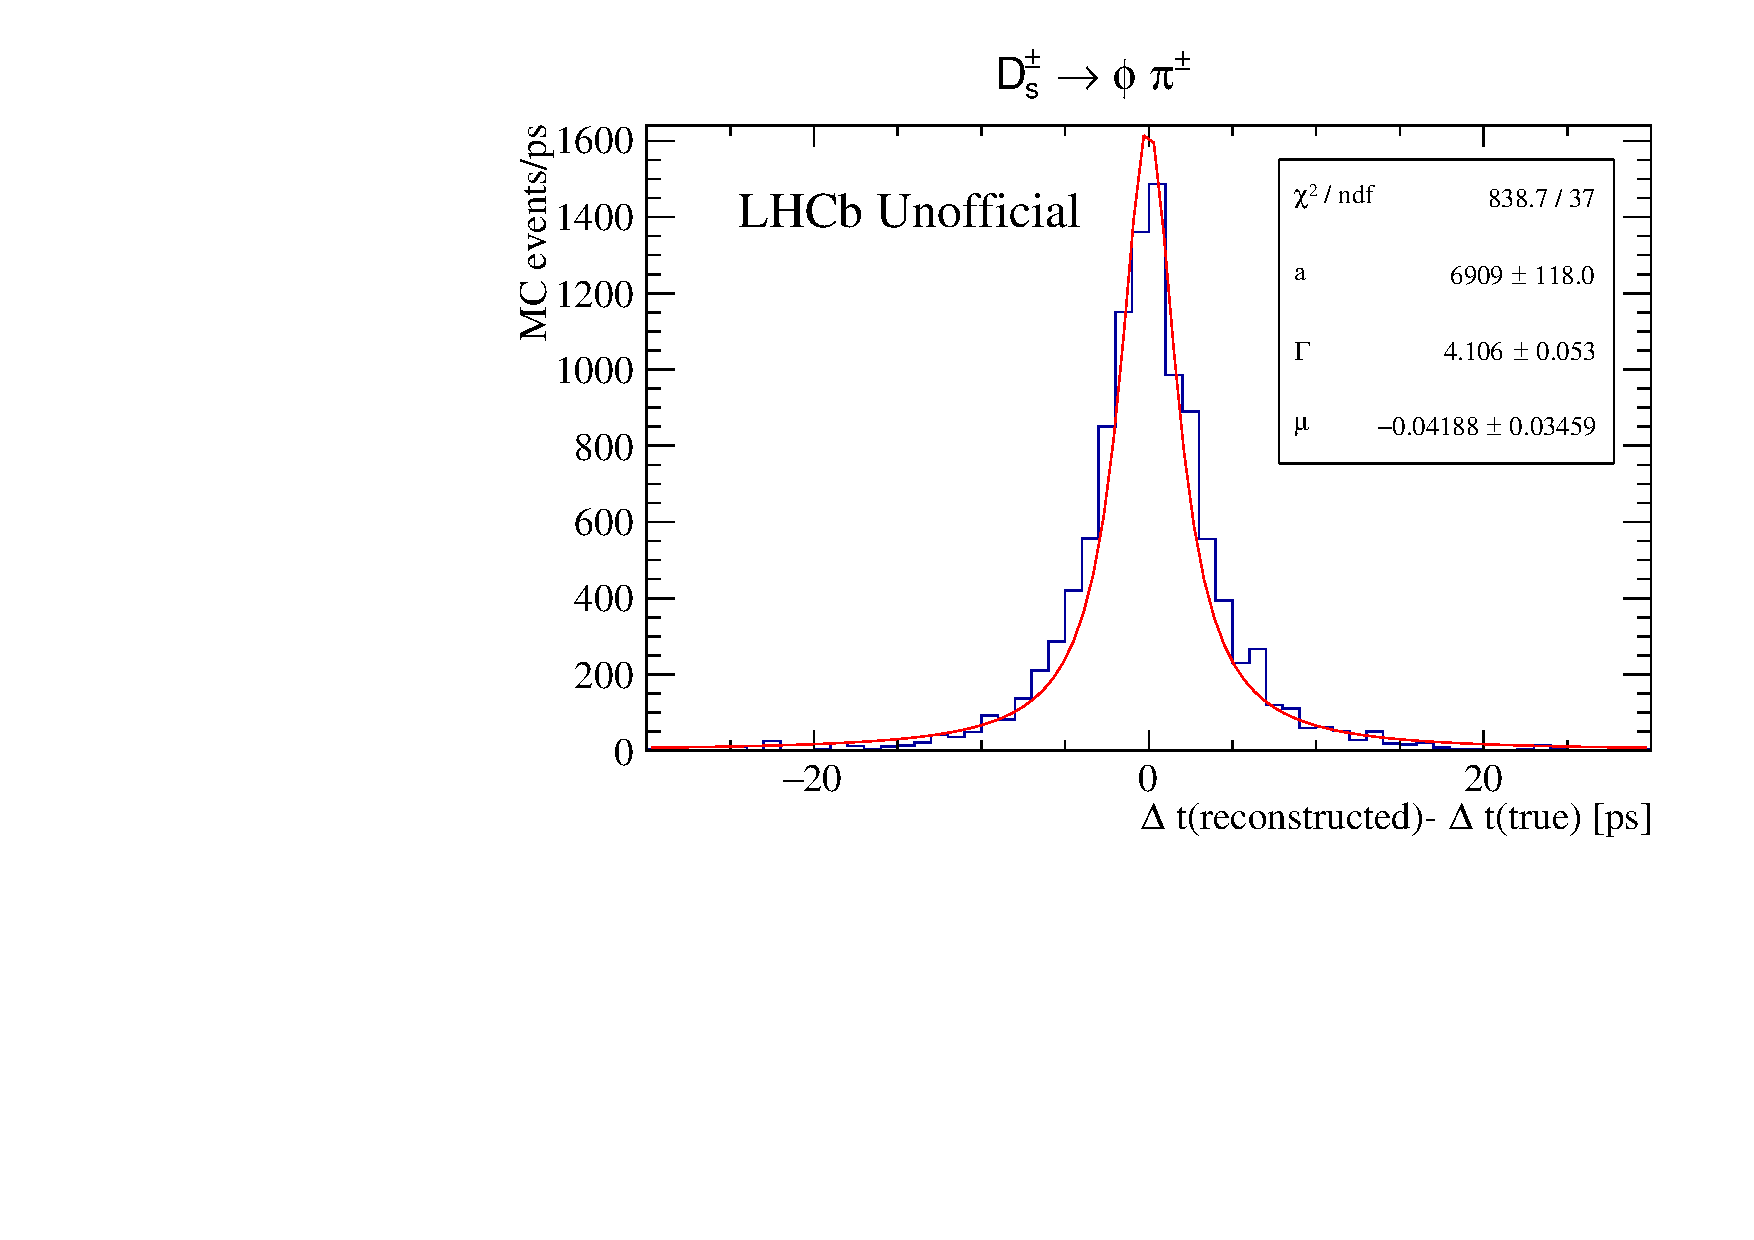
\includegraphics[width=.49\textwidth]{figs/time_res_Ds/timeResolution-DeltaTauLD.pdf}
\captionof{figure}{Resolution of $\Delta t$ for LL and DD kaons reconstructed using the TupleToolPropertime. }\label{FIG:LD-diff}
\end{center}

For the $D_s^\pm \rightarrow \phi \pi^\pm$ case, the width of the resolution of the decay time difference is smaller than for the actual decay times since the $\phi$ lifetime is negligible and therefore the residuals of the kaon decay times are correlated through the common ``vertex'' $D_s^\pm \rightarrow K^0 \overline{K}^0 \pi^\pm$ as can be seen in figure \ref{FIG:correlation}.

\begin{center}
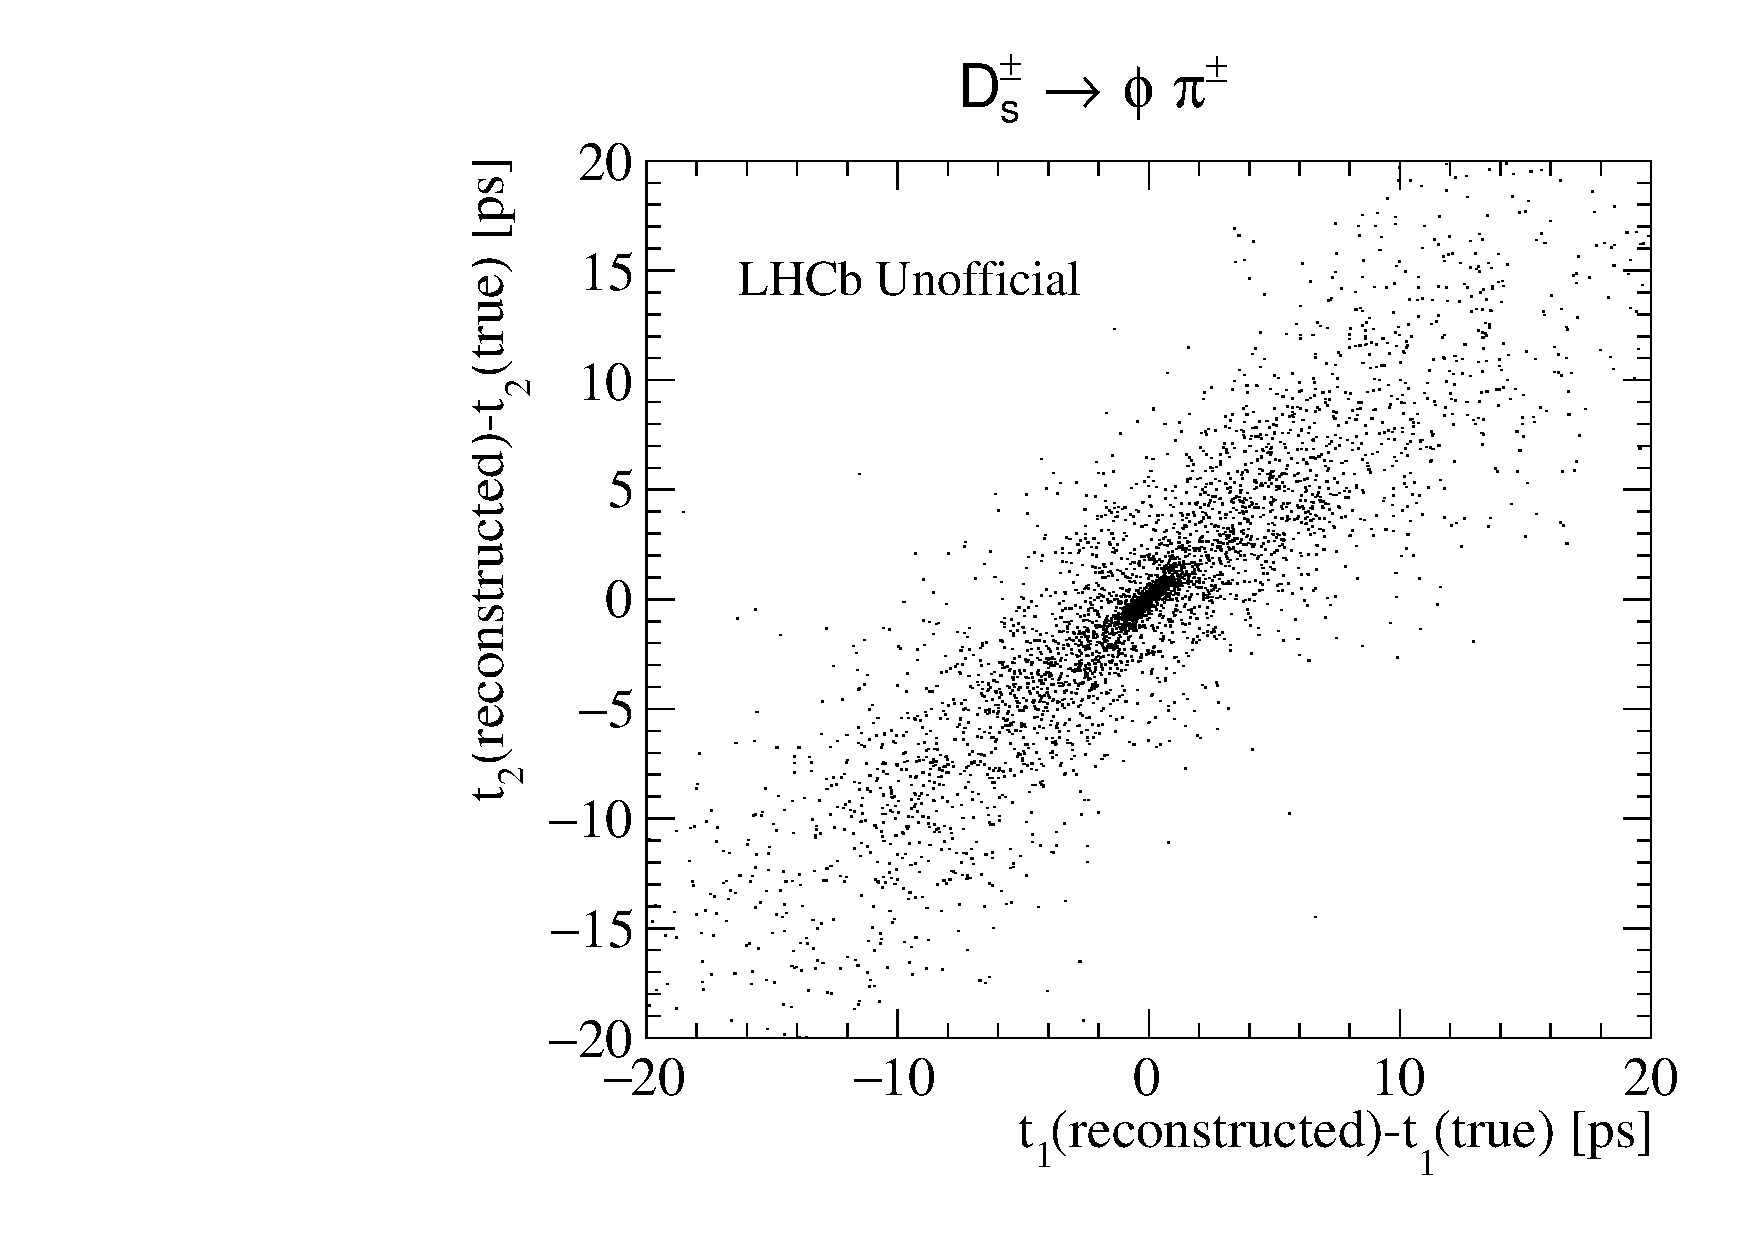
\includegraphics[width=.7\textwidth]{figs/time_res_Ds/UReco_2D.pdf}
\captionof{figure}{Correlation between the decay time residuals of both neutral kaons due to the common origin vertex.}\label{FIG:correlation}
\end{center}



